\section{Generazione del Codice Intermedio}

In questa fase si considerano \textbf{3 aspetti} fondamentali:

\begin{itemize}
    \item \textbf{Rappresentazione intermedia}, che si divide in:
    \begin{itemize}
        \item Alberi sintattici / DAG
        \item Codice a 3 indirizzi
    \end{itemize}
    \item \textbf{Analisi sintattica} (controlli di tipo).
    \item \textbf{Generazione del codice intermedio}.
\end{itemize}

\subsection*{Flusso di compilazione (Front-end vs Back-end)}
Il seguente schema illustra il flusso dei dati attraverso i componenti del compilatore:

\begin{center}
\begin{tikzpicture}[
    node distance=1cm and 1cm,
    auto,
    block/.style={
        rectangle, 
        draw, 
        text width=2cm, 
        align=center, 
        minimum height=3em
    },
    line/.style={draw, -latex}
]

    % Nodi
    \node (start) {};
    \node [block, right=0.5cm of start] (parser) {Parser};
    \node [block, right=of parser] (checker) {Checker\\statico};
    \node [block, right=of checker] (gen_int) {Generatore\\di codice\\intermedio};
    \node [block, right=2.5cm of gen_int] (gen_cod) {Generatore\\di codice};
    \node [right=0.5cm of gen_cod] (end) {};

    % Frecce
    \path [line] (start) -- (parser);
    \path [line] (parser) -- (checker);
    \path [line] (checker) -- (gen_int);
    \path [line] (gen_int) -- node [above, font=\footnotesize] {codice} node [below, font=\footnotesize] {intermedio} (gen_cod);
    \path [line] (gen_cod) -- (end);

    % Linee Front-end / Back-end
    % Linea orizzontale sotto
    \draw [thin] ($(parser.south west) + (0,-0.8)$) -- ($(gen_cod.south east) + (0,-0.8)$);
    
    % Separatore verticale
    \draw [thick] ($(gen_int.south east) + (1.25,-0.7)$) -- ($(gen_int.south east) + (1.25,-0.9)$);
    
    % Etichette
    \node [font=\footnotesize] at ($(checker.south) + (0.5,-1.1)$) {front-end};
    \node [font=\footnotesize] at ($(gen_cod.south) + (-0.5,-1.1)$) {back-end};

\end{tikzpicture}
\end{center}

\subsection{Analisi Statica (Static Checker)}
L'analisi statica è un insieme di controlli di consistenza effettuati al momento della compilazione per garantire che il programma possa essere compilato con successo e per individuare errori prima dell'esecuzione. Si divide in:

\subsubsection{1. Controlli Sintattici}
Verificano il rispetto delle regole strutturali del linguaggio. Esempi:
\begin{itemize}
    \item Un identificatore deve essere dichiarato al più una volta nello stesso scope.
    \item Un'istruzione \texttt{break} deve trovarsi all'interno di un ciclo (\texttt{while}, \texttt{for}) o \texttt{switch}.
    \item Distinzione tra \textbf{L-value} e \textbf{R-value}:
    \begin{itemize}
        \item \textbf{L-value} (Left-value): Indica una locazione di memoria (es. a sinistra di un assegnamento: \texttt{i = 5}).
        \item \textbf{R-value} (Right-value): Indica il valore contenuto nella locazione (es. a destra di un assegnamento: \texttt{x = i + 1}).
    \end{itemize}
\end{itemize}

\subsubsection{2. Controlli di Tipo}
Garantiscono che operatori e funzioni siano applicati a un numero corretto di operandi e che il loro tipo sia adeguato.
\begin{itemize}
    \item Esempio di conversione implicita (coercion):
    \begin{itemize}
        \item \texttt{x = 4 + 5} : Nessuna conversione necessaria.
        \item \texttt{x = 4 + 5.1} : Il numero intero \texttt{4} deve essere convertito in float prima della somma.
    \end{itemize}
\end{itemize}

\subsection{Rappresentazioni Intermedie e DAG}

La rappresentazione intermedia serve da ponte tra il front-end e il back-end. Esistono diversi livelli di astrazione:

\begin{center}
\begin{tikzpicture}[node distance=0.5cm, auto, font=\small]
    % Nodi del flusso
    \node (src) {Prog. Sorgente};
    \node[right=0.8cm of src] (high) {Rapp. Alto Livello};
    \node[right=0.8cm of high] (dots) {$\dots$};
    \node[right=0.8cm of dots] (low) {Rapp. Basso Livello};
    \node[right=0.8cm of low] (tgt) {Codice Target};

    % Frecce flusso
    \draw[->] (src) -- (high);
    \draw[->] (high) -- (dots);
    \draw[->] (dots) -- (low);
    \draw[->] (low) -- (tgt);

    % Annotazioni (Albero e 3 Indirizzi)
    \node[below=0.8cm of high, text=magenta] (tree_label) {Albero Sintattico};
    \draw[->, magenta, bend right] (tree_label.north) to (high.south);

    \node[below=0.8cm of low, text=magenta] (addr_label) {Codice a 3 indirizzi};
    \node[below=0.1cm of addr_label, font=\scriptsize] {$x = y \text{ op } z$};
    \draw[->, magenta, bend right] (addr_label.north) to (low.south);
\end{tikzpicture}
\end{center}

\begin{itemize}
    \item \textbf{Albero Sintattico:} Rappresentazione gerarchica fedele alla grammatica.
    \item \textbf{DAG (Grafo Aciclico Diretto):} Simile all'albero sintattico, ma identifica le sotto-espressioni comuni. I nodi con lo stesso valore/struttura vengono riutilizzati (parte condivisa).
\end{itemize}

\subsubsection*{Esempio di DAG}
Consideriamo l'espressione: $a + a * (b - c) + (b - c) * d$.
La sotto-espressione $(b - c)$ viene calcolata una sola volta e il nodo risultante viene puntato da entrambe le parti che lo utilizzano.

\begin{center}
\begin{tikzpicture}[
    level distance=1.5cm,
    sibling distance=1.5cm,
    every node/.style={circle, inner sep=1pt},
    edge from parent/.style={draw, thick}
]

    % Definizione manuale dei nodi per creare la condivisione
    \node (root) at (0,0) {$+$};
    
    \node (plus_left) at (-2, -1.5) {$+$};
    \node (mult_right) at (2, -1.5) {$*$};
    
    \node (a_first) at (-3, -3) {$a$};
    \node (mult_left) at (-1, -3) {$*$};
    \node (d) at (3, -3) {$d$};
    
    \node (a_second) at (-2, -4.5) {$a$};
    
    % Nodo condiviso (evidenziato in rosa come negli appunti)
    \node (minus_shared) at (0, -4.5) {$-$};
    \node (b) at (-0.5, -6) {$b$};
    \node (c) at (0.5, -6) {$c$};

    % Cerchio rosa attorno alla parte condivisa
    \draw[magenta, thick] (0, -5.2) ellipse (1cm and 1.5cm);
    \node[magenta, below=1.5cm of minus_shared] {$\uparrow$ parte condivisa};

    % Collegamenti
    \draw (root) -- (plus_left);
    \draw (root) -- (mult_right);
    
    \draw (plus_left) -- (a_first);
    \draw (plus_left) -- (mult_left);
    
    \draw (mult_right) -- (minus_shared); % Condivisione destra
    \draw (mult_right) -- (d);
    
    \draw (mult_left) -- (a_second);
    \draw (mult_left) -- (minus_shared); % Condivisione sinistra
    
    \draw (minus_shared) -- (b);
    \draw (minus_shared) -- (c);

\end{tikzpicture}
\end{center}

%lezione 26 novembre
\subsection{Grafi diretti aciclici delle espressioni}

\subsubsection{Definizione guidata dalla sintassi per la costruzione di alberi sintattici e DAG}

Per costruire un grafo si utilizzano le funzioni costruttore \texttt{Leaf} e \texttt{Node}.
Per esempio, prima di costruire un nuovo nodo $Node(op, left, right)$, dobbiamo verificare se esiste un nodo con etichetta $op$ e con figli $left$ e $right$, in quest'ordine. Se tale nodo esiste la funzione $Node()$ lo restituisce, altrimenti ne crea uno nuovo.

\begin{center}
\begin{tabular}{lll}
\hline
& \textbf{Produzione} & \textbf{Regole semantiche} \\
\hline
1) & $E \to E_1 + T$ & $E.node = \textbf{new } Node('+', E_1.node, T.node)$ \\
2) & $E \to E_1 - T$ & $E.node = \textbf{new } Node('-', E_1.node, T.node)$ \\
3) & $E \to T$ & $E.node = T.node$ \\
4) & $T \to ( E )$ & $T.node = E.node$ \\
5) & $T \to \textbf{id}$ & $T.node = \textbf{new } Leaf(\textbf{id}, \textbf{id}.entry)$ \\
6) & $T \to \textbf{num}$ & $T.node = \textbf{new } Leaf(\textbf{num}, \textbf{num}.val)$ \\
\hline
\end{tabular}
\end{center}

\subsubsection{Esempio 6.2: Costruzione di un DAG complesso}

La sequenza di passi indicati di seguito costruisce il DAG mostrato nella figura successiva, a patto che le funzioni $Leaf()$ e $Node()$ ritornino un nodo già esistente, secondo quanto appena discusso, quando ciò è possibile.
Consideriamo l'espressione:
\[ a + a * (b - c) + (b - c) * d \]
\begin{figure}[H]
    \centering
    \begin{tikzpicture}[
        node distance=1.5cm,
        every node/.style={circle, draw, minimum size=0.9cm, inner sep=0pt},
        level 1/.style={sibling distance=7cm},
        level 2/.style={sibling distance=3.5cm},
        level 3/.style={sibling distance=2cm}
    ]
        % --- LIVELLO 0 (Radice) ---
        \node (p13) at (0, 0) {+};
        \node[draw=none, right=0.3cm of p13] {$p_{13}$};

        % --- LIVELLO 1 ---
        % Nodo + a sinistra
        \node (p7) at (-3.5, -1.5) {+};
        \node[draw=none, left=0.3cm of p7] {$p_7$};

        % Nodo * a destra (CORRETTO: p12)
        \node (p12) at (3.5, -1.5) {*};
        \node[draw=none, right=0.3cm of p12] {$p_{12}$};

        % --- LIVELLO 2 ---
        % Sotto p7 (+)
        \node (p1) at (-5, -3) {\textbf{a}};
        \node[draw=none, left=0.3cm of p1] {$p_1$};

        \node (p6) at (-2, -3) {*};
        \node[draw=none, right=0.3cm of p6] {$p_6$};

        % Sotto p12 (*)
        \node (p10) at (2, -3) {-};
        \node[draw=none, right=0.3cm of p10] {$p_{10}$};

        % Nodo d (CORRETTO: p11)
        \node (p11) at (5, -3) {\textbf{d}};
        \node[draw=none, right=0.3cm of p11] {$p_{11}$};

        % --- LIVELLO 3 ---
        % Sotto p6 (*)
        \node (p2) at (-3, -4.5) {\textbf{a}};
        \node[draw=none, below=0.1cm of p2] {$p_2$};

        % Nodo - di sinistra (CORRETTO: p5)
        \node (p5) at (-1, -4.5) {-};
        \node[draw=none, right=0.3cm of p5] {$p_5$};

        % Sotto p10 (-)
        % Nodo b di destra (CORRETTO: p8)
        \node (p8) at (1, -4.5) {\textbf{b}};
        \node[draw=none, below=0.1cm of p8] {$p_8$};

        \node (p9) at (3, -4.5) {\textbf{c}};
        \node[draw=none, right=0.3cm of p9] {$p_9$};

        % --- LIVELLO 4 ---
        % Sotto il nodo - di sinistra (p5)
        \node (p3) at (-2, -6) {\textbf{b}};
        \node[draw=none, below=0.1cm of p3] {$p_3$};

        \node (p4) at (0, -6) {\textbf{c}};
        \node[draw=none, below=0.1cm of p4] {$p_4$};

        % --- ARCHI ---
        \draw (p13) -- (p7);
        \draw (p13) -- (p12);

        \draw (p7) -- (p1);
        \draw (p7) -- (p6);

        \draw (p12) -- (p10);
        \draw (p12) -- (p11);

        \draw (p6) -- (p2);
        \draw (p6) -- (p5);

        \draw (p10) -- (p8);
        \draw (p10) -- (p9);

        \draw (p5) -- (p3);
        \draw (p5) -- (p4);

    \end{tikzpicture}
    \caption{L'Albero Sintattico per l'espressione $a + a * (b - c) + (b - c) * d$ senza condivisione.}
\end{figure}

Assumiamo che $entry\text{-}a$ sia un puntatore all'elemento della tabella dei simboli relativo ad \textbf{a}, e così per gli altri identificatori. Alla seconda invocazione di $Leaf(\textbf{id}, entry\text{-}a)$, alla linea 2, la funzione restituisce il puntatore al nodo precedentemente costruito, ovvero $p_2 = p_1$. Analogamente, i nodi restituiti ai passi 8 e 9 coincidono con quelli restituiti ai passi 3 e 4 (cioè $p_8 = p_3$ e $p_9 = p_4$). Di conseguenza, il nodo restituito al passo 10 deve essere lo stesso restituito al passo 5, cioè $p_{10} = p_5$.

\bigskip
\textbf{Sequenza dei puntatori:}
\begin{enumerate}
    \item $p_1 = Leaf(\textbf{id}, entry\text{-}a)$
    \item $p_2 = Leaf(\textbf{id}, entry\text{-}a) = p_1$
    \item $p_3 = Leaf(\textbf{id}, entry\text{-}b)$
    \item $p_4 = Leaf(\textbf{id}, entry\text{-}c)$
    \item $p_5 = Node('-', p_3, p_4)$
    \item $p_6 = Node('*', p_1, p_5)$
    \item $p_7 = Node('+', p_1, p_6)$
    \item $p_8 = Leaf(\textbf{id}, entry\text{-}b) = p_3$
    \item $p_9 = Leaf(\textbf{id}, entry\text{-}c) = p_4$
    \item $p_{10} = Node('-', p_3, p_4) = p_5$
    \item $p_{11} = Leaf(\textbf{id}, entry\text{-}d)$
    \item $p_{12} = Node('*', p_5, p_{11})$
    \item $p_{13} = Node('+', p_7, p_{12})$
\end{enumerate}

\bigskip
\textbf{L'Albero Sintattico (DAG) diventa:}

\begin{figure}[h!]
    \centering
    \begin{tikzpicture}[
        node distance=1.5cm,
        every node/.style={circle, draw, minimum size=0.9cm, inner sep=0pt},
        level 1/.style={sibling distance=5cm},
        level 2/.style={sibling distance=3cm}
    ]
        % Livello Radice (p13)
        \node (p13) at (0,0) {+}; 
        \node[draw=none, right=0.2cm of p13] {$p_{13}$};

        % Livello 1 (p7, p12)
        \node (p7) at (-2.5,-1.5) {+}; 
        \node[draw=none, left=0.2cm of p7] {$p_7$};
        
        \node (p12) at (2.5,-1.5) {*}; 
        \node[draw=none, right=0.2cm of p12] {$p_{12}$};

        % Livello 2 (a, p6, d)
        \node (a) at (-4,-3) {\textbf{a}}; 
        \node[draw=none, left=0.2cm of a] {$p_1, p_2$};
        
        \node (p6) at (-1,-3) {*}; 
        \node[draw=none, right=0.2cm of p6] {$p_6$};
        
        \node (d) at (4,-3) {\textbf{d}}; 
        \node[draw=none, right=0.2cm of d] {$p_{11}$};

        % Livello 3 (Nodo condiviso p5)
        \node (p5) at (1.5,-4.5) {-}; 
        \node[draw=none, right=0.2cm of p5] {$p_5, p_{10}$};

        % Livello 4 (Foglie condivise b, c)
        \node (b) at (0,-6) {\textbf{b}}; 
        \node[draw=none, left=0.2cm of b] {$p_3, p_8$};
        
        \node (c) at (3,-6) {\textbf{c}}; 
        \node[draw=none, right=0.2cm of c] {$p_4, p_9$};

        % Archi
        \draw (p13) -- (p7);
        \draw (p13) -- (p12);
        
        \draw (p7) -- (a);
        \draw (p7) -- (p6);
        
        \draw (p12) -- (p5);
        \draw (p12) -- (d);
        
        \draw (p6) -- (a); % Riuso di a
        \draw (p6) -- (p5); % Riuso di b-c
        
        \draw (p5) -- (b);
        \draw (p5) -- (c);

    \end{tikzpicture}
    \caption{DAG per l'espressione $a + a * (b - c) + (b - c) * d$.}
\end{figure}

\vspace{1 cm}
\subsection{Metodo del valore numerico per la costruzione di DAG}

Come suggerito dalla figura seguente, i nodi di un albero sintattico sono spesso memorizzati in un \textbf{Array di Record}. Ogni riga dell'array rappresenta un record e quindi un nodo. In ogni record, il primo campo è un codice operativo che indica l'etichetta del nodo.
Le foglie hanno un campo aggiuntivo contenente il valore lessicale; i nodi interni hanno due campi aggiuntivi che rappresentano i figli sinistro e destro.

In questo array ci riferiamo ai nodi mediante l'indice del record corrispondente al nodo d'interesse. Storicamente, tale indice è stato chiamato \textbf{valore numerico} o \textit{value number} del nodo o dell'espressione che esso rappresenta.
Chiamiamo \textbf{Firma (Signature)} di un nodo interno la tripla $\langle op, l, r \rangle$, in cui $op$ è l'etichetta, $l$ il valore numerico del figlio sinistro e $r$ quello del figlio destro.

\vspace{3 cm}
\textbf{Esempio:} $i = i + 10$

\begin{figure}[h!]
    \centering
    \begin{minipage}{0.45\textwidth}
        \centering
        \begin{tikzpicture}[node distance=1.5cm, auto, >=latex]
            \node[circle, draw] (eq) {=};
            \node[circle, draw, below right=of eq] (plus) {+};
            \node[draw=none, below left=of eq] (i) {i};
            \node[draw=none, below right=of plus] (ten) {10};

            \draw[->] (eq) to [bend right] (i);
            \draw[->] (eq) -- (plus);
            \draw[->] (plus) -- (i);
            \draw[->] (plus) -- (ten);
        \end{tikzpicture}
        \caption{(a) DAG}
    \end{minipage}
    \hfill
    \begin{minipage}{0.45\textwidth}
        \centering
        \begin{tabular}{|c|c|c|c|}
        \hline
        1 & \textbf{id} & \multicolumn{2}{c|}{$i$} \\ \hline
        2 & \textbf{num} & \multicolumn{2}{c|}{10} \\ \hline
        3 & + & 1 & 2 \\ \hline
        4 & = & 1 & 3 \\ \hline
        \end{tabular}
        \caption{(b) Array}
    \end{minipage}
    \caption{Nodi del DAG di $i = i + 10$ allocati in un array.}
\end{figure}

\subsubsection{Algoritmo 6.3}

\textbf{Algoritmo 6.3: Metodo del valore numerico per la costruzione dei nodi di un DAG.}

\begin{itemize}
    \item \textbf{INPUT:} L'etichetta $op$, il nodo $l$ e il nodo $r$.
    \item \textbf{OUTPUT:} Il valore numerico di un nodo nell'array con firma $\langle op, l, r \rangle$.
    \item \textbf{METODO:} Si cerchi nell'array un nodo $M$ con etichetta $op$, figlio sinistro $l$ e figlio destro $r$. Se un tale nodo esiste, si restituisca il valore numerico di $M$. Altrimenti si crei un nuovo nodo $N$ con etichetta $op$, figlio sinistro $l$ e figlio destro $r$ e si restituisca il suo valore numerico.
\end{itemize}

\subsubsection{Struttura dati per la ricerca (Tabella Hash)}

Per costruire una tabella di hash per i nodi di un DAG, abbiamo bisogno di una \textit{funzione di hash} che calcola l'indice del gruppo data una firma $\langle op, l, r \rangle$ in maniera tale da distribuire il più uniformemente possibile le firme nei vari gruppi.
Un array, indicizzato in base al valore della funzione di hash, contiene i puntatori alle teste delle varie liste.

\begin{figure}[h!]
    \centering
    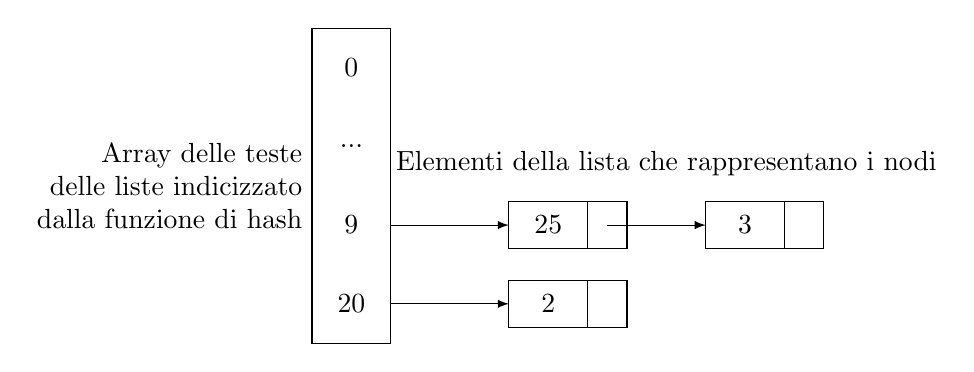
\begin{tikzpicture}
        % Array delle teste (Bucket)
        \draw (0,0) rectangle (1,4);
        \node at (0.5, 3.5) {0};
        \node at (0.5, 2.5) {...};
        \node at (0.5, 1.5) {9};
        \node at (0.5, 0.5) {20};
        \node[left, align=right] at (0, 2) {Array delle teste\\delle liste indicizzato\\dalla funzione di hash};
        
        % Bucket 9 punta alla lista
        \draw[-latex] (1, 1.5) -- (2.5, 1.5);
        \draw (2.5, 1.2) rectangle (3.5, 1.8) node[midway] {25};
        \draw (3.5, 1.2) rectangle (4.0, 1.8); 
        \draw[-latex] (3.75, 1.5) -- (5.0, 1.5);
        \draw (5.0, 1.2) rectangle (6.0, 1.8) node[midway] {3};
        \draw (6.0, 1.2) rectangle (6.5, 1.8); 
        
        % Bucket 20 punta alla lista
        \draw[-latex] (1, 0.5) -- (2.5, 0.5);
        \draw (2.5, 0.2) rectangle (3.5, 0.8) node[midway] {2};
        \draw (3.5, 0.2) rectangle (4.0, 0.8);
        
        \node[above] at (4.5, 2) {Elementi della lista che rappresentano i nodi};
    \end{tikzpicture}
    \caption{Struttura dati per la ricerca degli elementi in un gruppo.}
\end{figure}

La ricerca del VN di una firma $\langle op, l, r \rangle$ procede cercando il nodo richiesto all'interno della lista $h(\langle op, l, r \rangle)$.
\begin{itemize}
    \item Si scorre la lista alla ricerca di un elemento la cui firma sia $\langle op, l, r \rangle$.
    \item \textbf{SE} si trova un tale elemento, se ne restituisce il valore numerico.
    \item \textbf{ALTRIMENTI}, si aggiunge alla lista un elemento con firma $\langle op, l, r \rangle$ e se ne restituisce il VN.
\end{itemize}

\subsection{Codice a 3 Indirizzi}

Esempio:
\begin{verbatim}
x = y op z
x + y * z
    t1 = y * z
    t2 = x + t1
\end{verbatim}

Il seguente codice a tre indirizzi è derivato direttamente dalla struttura del DAG mostrato sopra. Notare come le variabili temporanee riutilizzino i risultati comuni (come $t_1$).

\begin{verbatim}
t1 = b - c
t2 = a * t1
t3 = a + t2
t4 = t1 * d
t5 = t3 + t4
\end{verbatim}

Consideriamo ora le più comuni istruzioni a tre indirizzi che utilizzeremo nel resto di questa trattazione.
Un indirizzo può assumere una delle seguenti forme:
\begin{enumerate}
    \item \textbf{Un nome.} Per comodità, nel codice a tre indirizzi utilizzeremo direttamente i nomi degli identificatori così come appaiono nel codice sorgente.
    \item \textbf{Una costante.} In pratica un compilatore deve trattare molti tipi diversi di costanti e variabili.
    \item \textbf{Un nome temporaneo} generato dal compilatore, ogni volta che una variabile temporanea sia necessaria.
\end{enumerate}

\subsubsection{Le istruzioni più comuni}

\begin{enumerate}
    \item \textbf{Istruzioni di assegnamento del tipo $x = y \ op \ z$}, in cui $op$ è un operatore binario aritmetico o logico e $x$, $y$ e $z$ sono indirizzi.
    
    \item \textbf{Istruzioni di assegnamento del tipo $x = op \ z$}, in cui $op$ indica un'operazione unaria. (Es. meno unario, la negazione logica.)
    
    \item \textbf{Istruzioni di copia del tipo $x = y$}, secondo cui a $x$ viene assegnato il valore di $y$.
    
    \item \textbf{Istruzioni di salto incondizionato del tipo \texttt{goto L}}, secondo cui la successiva istruzione a essere eseguita sarà quella con etichetta simbolica $L$.
    
    \item \textbf{Istruzioni di salto condizionato del tipo \texttt{if x goto L} oppure \texttt{ifFalse x goto L}}. Queste istruzioni fanno sì che l'istruzione successiva a essere eseguita sia quella indicata dall'etichetta $L$ se la condizione $x$ è rispettivamente vera oppure falsa. In entrambi i casi, qualora la condizione non sia soddisfatta sarà l'istruzione immediatamente successiva a essere eseguita, seguendo pertanto il normale flusso di esecuzione.
    
    \item \textbf{Istruzioni di salto condizionato del tipo \texttt{if x relop y goto L}}. Tali istruzioni applicano l'operatore relazionale $relop$ ($<, \le, ==, \dots$) agli operandi $x$ e $y$; se tali operandi soddisfano la relazione indicata esse fanno sì che la successiva istruzione a essere eseguita sia quella con etichetta $L$. In caso contrario, sarà l'istruzione immediatamente successiva a essere eseguita, seguendo pertanto il normale flusso di esecuzione.
    
    \item \textbf{Chiamata di procedura e ritorno da procedura.} Le chiamate di procedura sono implementate mediante una istruzione \texttt{param x} per ogni parametro, una istruzione \texttt{call p, n} oppure \texttt{y = call p, n} per la chiamata vera e propria della procedura o della funzione e, infine, una istruzione \texttt{return y} -- in cui l'indirizzo $y$ è opzionale -- che indica il valore restituito al chiamante.
    \\
    Generata in corrispondenza della chiamata di procedura $p(x_1, x_2, \dots, x_n)$. Il valore intero $n$, che indica il numero dei parametri in una chiamata del tipo \texttt{call p, n}, non è ridondante, poiché le chiamate possono essere annidate. In altre parole può accadere che alcune delle prime istruzioni \texttt{param} siano parte di una chiamata che avviene dopo che $p$ ha restituito il suo valore, che diviene pertanto un ulteriore parametro per la seconda chiamata. 
    
    \item \textbf{Istruzioni di copia indicizzata del tipo $x = y[i]$ oppure $x[i] = y$}. La prima istruzione assegna a $x$ il valore che si trova $i$ posizioni dopo la locazione di memoria indicata da $y$. Analogamente, la seconda istruzione assegna il valore $y$ alla locazione di memoria che si trova $i$ posizioni dopo quella relativa a $x$.
    
    \item \textbf{Assegnamenti di puntatori e indirizzi del tipo $x = \&y$, $x = *y$ oppure $*x = y$}. 
    L'istruzione $x = \&y$ assegna a $x$, precisamente all'r-value di $x$, l'indirizzo di $y$, cioè il suo l-value. Presumibilmente $y$ è un nome, eventualmente temporaneo, che denota una espressione avente un l-value definito, come \texttt{A[i][j]}, mentre $x$ è il nome di un puntatore oppure una variabile temporanea. 
    Nell'istruzione $x = *y$, presumibilmente $y$ è un puntatore o una variabile temporanea il cui r-value indica una locazione di memoria; in tal caso $x$ (il suo r-value) assume il valore di tale locazione. 
    Infine, l'istruzione $*x = y$ assegna il valore di $y$ all'r-value dell'oggetto puntato da $x$.
\end{enumerate}


%lezione 27 novembre
\textbf{Esempio 6.5.} Si consideri lo statement:
$$ do \ i = i + 1; \ while \ (a[i] < v); $$

Due possibili traduzioni sono mostrate nella figura seguente. La soluzione (a) utilizza un'etichetta simbolica $L$ associata alla prima istruzione. La traduzione (b) utilizza i numeri delle posizioni delle istruzioni, iniziando arbitrariamente a 100. In entrambi i casi l'ultima istruzione è un salto condizionato alla prima istruzione.

\subsubsection*{Nota}
La moltiplicazione $i * 8$ sottintende che la dimensione di ogni elemento dell'array abbia dimensioni pari a 8 unità.


\begin{table}[H]
\centering
\begin{tabular}{l|l}
\textbf{(a) Etichette simboliche} & \textbf{(b) Indici di posizione} \\
\hline
\begin{minipage}{6cm}
\vspace{0.2cm}
L: \quad $t_1 = i + 1$ \\
\hspace*{0.6cm} $i = t_1$ \\
\hspace*{0.6cm} $t_2 = i * 8$ \\
\hspace*{0.6cm} $t_3 = a[t_2]$ \\
\hspace*{0.6cm} if $t_3 < v \ goto \ L$
\vspace{0.2cm}
\end{minipage}
&
\begin{minipage}{6cm}
\vspace{0.2cm}
100: \ $t_1 = i + 1$ \\
101: \ $i = t_1$ \\
102: \ $t_2 = i * 8$ \\
103: \ $t_3 = a[t_2]$ \\
104: \ if $t_3 < v \ goto \ 100$
\vspace{0.2cm}
\end{minipage}
\end{tabular}
\caption{Due metodi per l'assegnamento delle etichette a una sequenza di istruzioni a tre indirizzi }
\end{table}

La scelta di quali operatori utilizzare nella rappresentazione intermedia è cruciale. L'insieme deve essere sufficientemente ricco da consentire l'implementazione di tutte le operazioni del linguaggio sorgente.

\subsection{Rappresentazione del Codice Intermedio}

Le istruzioni a tre indirizzi possono essere implementate come record. Tre comuni rappresentazioni sono le \textbf{quadruple}, le \textbf{triple} e le \textbf{triple indirette}.

\subsubsection{1. Quadruple}
Una quadrupla (o \textit{quad}) ha quattro campi: $op$, $arg_1$, $arg_2$ e $result$.
Il campo $op$ contiene un codice interno che indica l'operatore.
Esempio: $x = y + z$ è rappresentato con $+$, $y$, $z$, $x$.

\textbf{Eccezioni:}
\begin{itemize}
    \item Istruzioni con operatori unari (es. $x = \text{minus } y$) o copie ($x=y$) non usano $arg_2$. Per le copie, $op$ è l'assegnamento.
    \item Istruzioni come $param \ x$ non usano né $arg_2$ né $result$.
    \item I salti condizionati e incondizionati salvano l'etichetta in $result$.
\end{itemize}

\textbf{Esempio:} $a = b * -c + b * -c$

\begin{table}[H]
\centering
\begin{tabular}{|c|c|c|c|c|}
\hline
 & \textbf{op} & \textbf{arg$_1$} & \textbf{arg$_2$} & \textbf{result} \\
\hline
0 & minus & c & & $t_1$ \\
1 & * & b & $t_1$ & $t_2$ \\
2 & minus & c & & $t_3$ \\
3 & * & b & $t_3$ & $t_4$ \\
4 & + & $t_2$ & $t_4$ & $t_5$ \\
5 & = & $t_5$ & & a \\
\hline
\end{tabular}
\caption{Rappresentazione tramite Quadruple. Si nota come il "minus" unario sia distinto dalla sottrazione.}
\end{table}

\subsubsection{2. Triple}
Una tripla è un record con soli tre campi: $op$, $arg_1$ e $arg_2$.
Il campo $result$ è utilizzato principalmente da variabili temporanee, quindi viene eliminato. Ci si riferisce al risultato di un'operazione mediante la sua \textbf{posizione} nella sequenza di codice (es. $(0)$, $(1)$).

Le triple sono equivalenti alla struttura di un \textbf{DAG} (Albero Sintattico).

\begin{figure}[H]
\centering
\begin{minipage}{0.45\textwidth}
    \centering
    \begin{tikzpicture}[
        level distance=1.2cm, % Aumentato leggermente per leggibilità verticale
        level 1/.style={sibling distance=4cm}, % Molto spazio tra 'a' e il blocco '+'
        level 2/.style={sibling distance=2.5cm}, % Spazio tra i due '*' per evitare collisioni sotto
        level 3/.style={sibling distance=1.2cm}  % Spazio normale tra 'b' e 'minus'
    ]
    \node {=}
        child {node {a}}
        child {node {+}
            child {node {*}
                child {node {b}}
                child {node {minus} child {node {c}}}
            }
            child {node {*}
                child {node {b}}
                child {node {minus} child {node {c}}}
            }
        };
    \end{tikzpicture}
    \caption{Albero Sintattico}
    \end{minipage}
\hfill
\begin{minipage}{0.45\textwidth}
\centering
\begin{tabular}{|c|c|c|c|}
\hline
 & \textbf{op} & \textbf{arg$_1$} & \textbf{arg$_2$} \\
\hline
0 & minus & c & \\
1 & * & b & (0) \\
2 & minus & c & \\
3 & * & b & (2) \\
4 & + & (1) & (3) \\
5 & = & a & (4) \\
\hline
\end{tabular}
\caption{Tabella delle Triple }
\end{minipage}
\end{figure}

L'istruzione di copia $a=t_5$, nella notazione a triple è codificato ponendo $a$ in $arg_1$ e il valore numerico $(4)$ in $arg_2$.

\subsubsection{3. Triple Indirette}
Uno svantaggio delle triple, rispetto alle quadruple, emerge nei compilatori ottimizzanti. Se spostiamo un'istruzione, dobbiamo modificare tutti i riferimenti al suo indice.
Le \textbf{triple indirette} risolvono il problema usando una lista di puntatori alle triple (array \textit{instruction}).
L'ottimizzatore può spostare l'istruzione modificando l'ordine in \textit{instruction}, senza toccare le triple stesse.

\textbf{Esempio:} Istruzione $z = (x+y) * (10+w)$;

\vspace{0.5cm}

% Parte superiore: Confronto tra ordine originale e riordinato
\begin{center}
\begin{tabular}{p{3cm} c c c c}
\textbf{3 Istruzioni} & \textbf{Triple (Originali)} & & \textbf{Esecuzione Riordinata} & \\
$t_1: x+y$     & 0: + x y     & & + 10 w & \\
$t_2: 10+w$    & 1: + 10 w    & $\xrightarrow{\text{CAMBIO ORDINE}}$ & + x y & \\
$t_3: t_1 * t_2$ & 2: * (0) (1) & & * (1) (0) & \\
$z: t_3$       & 3: = z (2)   & & = z (2) & \\
\end{tabular}
\end{center}

\vspace{0.8cm}

% Parte inferiore: Array Instruction
\noindent \textbf{Array Instruction:}

\begin{center}
\begin{minipage}{0.2\textwidth}
    \centering
    (0) \\
    (1) \\
    (2) \\
    (3)
\end{minipage}
\begin{minipage}{0.1\textwidth}
    \centering
    $\longrightarrow$
\end{minipage}
\begin{minipage}{0.2\textwidth}
    \centering
    (1) \\
    (0) \\
    (2) \\
    (3)
\end{minipage}
\begin{minipage}{0.35\textwidth}
    \small $\rightarrow$ I puntatori nelle triple non cambiano, cambia solo l'ordine nell'array.
\end{minipage}
\end{center}

\subsection{Tipi e Dichiarazioni}

L'uso dei tipi ha diversi obiettivi, raggruppabili in due classi:

\begin{itemize}
    \item \textbf{Controllo di tipo (Type Checking):} Il controllo di tipo utilizza regole logiche per analizzare staticamente il comportamento di un programma al momento della sua esecuzione. Specificamente, garantisce che i tipi degli operandi siano quelli adatti al relativo operatore. 
    
    \item \textbf{Traduzione:} In base al tipo di un determinato nome, il compilatore può determinare lo spazio di memoria necessario a run-time. Inoltre, le informazioni di tipo sono necessarie per calcolare l'indirizzo relativo a un elemento di un array, per conversioni di tipo, ecc.
\end{itemize}

\vspace{0.3cm}

\noindent \textbf{Organizzazione della memoria:} La memoria per i nomi dichiarati all'interno di una procedura o di una classe è allocata durante l'esecuzione. Tuttavia, a compile-time, definiamo l'organizzazione ricorrendo a \textit{indirizzi relativi} (offset). L'indirizzo relativo è uno spiazzamento rispetto all'inizio della zona dati.

\subsubsection{Espressioni di Tipo}

I tipi hanno una struttura ben precisa che rappresenteremo mediante le \textit{espressioni di tipo}, di cui useremo la seguente definizione.
\begin{itemize}
    \item Un \textbf{tipo di base} è un'espressione di tipo (es. \textit{boolean, char, integer, float, void}).
    \item Un \textbf{nome di tipo} è un'espressione di tipo.
    \item Un'espressione di tipo può essere costruita applicando il costruttore di tipo \textbf{array} a un intero e a un'espressione di tipo.
    \item Un \textbf{record} è una struttura dati composta da campi aventi un nome. Si applica il costruttore \textit{record} ai nomi dei campi e ai loro tipi.
    \item Un'espressione può essere ottenuta applicando il costruttore di tipo $\rightarrow$ relativo ai tipi delle funzioni. Scriviamo $s \rightarrow t$ per indicare una funzione dal tipo $s$ (argomenti) al tipo $t$ (valore restituito).
    \item Se $s$ e $t$ sono espressioni di tipo, anche il loro \textbf{prodotto cartesiano} $s \times t$ è un'espressione di tipo.
    \begin{quote}
        \textit{\small $\rightarrow$ Nota : Serve per formare coppie e può essere usato più volte (es. liste o tuple).}
    \end{quote}
    \item Le espressioni di tipo possono contenere variabili i cui valori sono altre espressioni di tipo.
\end{itemize}

\vspace{0.5cm}

\subsubsection{Tipi Ricorsivi}
È un tipo di dato che fa riferimento a sé stesso nelle proprie definizioni.

$$ LIST = Nil \ | \ integer \times LIST $$

\noindent \textbf{Rappresentazione grafica (Grafo dei tipi):}

\begin{center}
\begin{tikzpicture}[>=Stealth, node distance=1.5cm, auto]
    % Stile dei nodi come nel disegno (ellissi)
    \node[draw, ellipse, thick, minimum width=1.5cm] (list) {LIST};
    \node[draw, ellipse, thick, minimum width=1cm, below left=1.5cm of list] (nil) {Nil};
    
    % Nodo prodotto cartesiano (cerchio con X)
    \node[draw, circle, thick, inner sep=2pt, below right=1.5cm of list] (cross) {$\times$};
    
    % Nodo integer
    \node[draw, ellipse, thick, minimum width=1.5cm, below=1.5cm of cross] (int) {integer};

    % Archi
    \draw[->, thick] (list) -- (nil);
    \draw[->, thick] (list) -- (cross);
    \draw[->, thick] (cross) -- (int);
    
    % Arco curvo di ritorno (ricorsione)
    \draw[->, thick] (cross) to[out=45, in=0] (list);
\end{tikzpicture}
\end{center}

\subsubsection{Equivalenza di Tipo}
Due espressioni di tipo sono strutturalmente equivalenti se e solo se:
\begin{enumerate}
    \item Sono lo stesso tipo di base.
    \item Sono ottenute applicando lo stesso costruttore di tipo a espressioni strutturalmente equivalenti a due a due.
    \item Una è un nome di tipo che indica l'altra.
\end{enumerate}
Se i nomi di tipo fossero interpretati come se rappresentassero loro stessi, le prime due condizioni della definizione appena citata portano al concetto di equivalenza per nome.


\subsubsection{Grammatica per le Dichiarazioni}

Studiamo i tipi utilizzando una grammatica semplificata, che dichiara un solo nome alla volta:

\begin{align*}
D &\to T \ id ; \ D \ | \ \epsilon \\
T &\to B \ C \ | \ record \ \{ D \} \\
B &\to int \ | \ float \\
C &\to [num] \ C \ | \ \epsilon
\end{align*}
\begin{itemize}
    \item Il non-terminale $D$ genera dichiarazioni.
    \item Il non-terminale $T$ genera tipi base, array e record.
    \item Il non-terminale $B$ genera uno dei due tipi di base (int e float).
    \item Il non-terminale $C$ (componente) genera stringhe di zero o più interi.
    \item Un tipo array consiste di un tipo di base specificato da B seguito dalle componenti descritte da C.
    \item Un tipo record (la seconda produzione relativa a T) è una sequenza di dichiarazioni relative ai diversi campi del record racchiuse tra parentesi graffe 
\end{itemize}    
    

\subsubsection{Organizzazione della Memoria per i nomi locali}
Dal nome di un tipo possiamo determinare la quantità di memoria che sarà necessaria a run-time per memorizzare valori associati a quel nome. A compile-time, possiamo utilizzare le informazioni relative al tipo per assegnare a ogni nome un indirizzo relativo.

Il tipo e l'indirizzo relativo di un certo nome sono memorizzati nell'elemento della tabella dei simboli relativo a quel nome. I dati di dimensione variabile (per esempio, le stringhe) o quelli la cui dimensione non può essere determinata se non al momento dell'esecuzione (per esempio, gli array dinamici) sono gestiti riservando solamente una quantità di memoria nota a priori e destinata a contenere un puntatore ai dati veri e propri.

Supponiamo che la memoria sia organizzata in blocchi contigui di più byte, nell'ipotesi che il byte sia la più piccola unità di memoria indirizzabile.

La \textit{larghezza} di un tipo indica il numero di unità di memorizzazione (\textbf{BYTE}) necessarie per un oggetto di quel tipo. I tipi di base (interi, caratteri, valori in virgola mobile) richiedono un numero intero di byte.

Per semplificare l'accesso, l'organizzazione della memoria relativa a tipi aggregati quali array e classi prevede un'allocazione contigua in un unico blocco.

\vspace{0.5cm}

\color{blue} % Colore blu per simulare la penna, opzionale (richiede package xcolor)
\textbf{ALLINEAMENTO:} \color{black}Porta ad un surplus di byte (\textit{PADDING}). \\
$\hookrightarrow$ ES: i 2 byte sprecati per allineare.
\color{black}

\vspace{0.5cm}


\subsubsection{SDT PER CALCOLARE IL TIPO (TYPE) E LA LARGHEZZA (WIDTH) PER I TIPI BASE E GLI ARRAY}

Lo SDT utilizza gli attributi sintetizzati $type$ e $width$ per ogni non-terminale e due variabili $t$ e $w$ per passare le informazioni di tipo e larghezza da un nodo $B$ nell'albero di parsing al nodo relativo alla produzione $C \to \epsilon$. In una definizione guidata dalla sintassi $t$ e $w$ sarebbero attributi ereditati di $C$.

\begin{align*}
T &\to B \quad \{ t = B.type; \ w = B.width; \} \\
  &\quad \ \ C \quad \{ T.type = C.type; \ T.width = C.width; \} \\[1em]
B &\to \mathbf{int} \quad \{ B.type = integer; \ B.width = 4; \} \\
B &\to \mathbf{float} \quad \{ B.type = float; \ B.width = 8; \} \\[1em]
C &\to \epsilon \quad \{ C.type = t; \ C.width = w; \} \\
C &\to [\mathbf{num}] \ C_1 \quad \{ C.type = array(\mathbf{num}.value, C_1.type); \\
  &\quad \quad \quad \quad \quad \quad \quad C.width = \mathbf{num}.value \times C_1.width; \}
\end{align*}

\vspace{0.3cm}
\noindent \textbf{Spiegazione:}
\begin{itemize}
    \item Il corpo della produzione per $T$ assegna $B.type$ a $t$ e $B.width$ a $w$.
    \item Le produzioni per $C$ determinano se $T$ genera un tipo base o un array.
    \item Se $C \to \epsilon$, allora $t$ e $w$ diventano gli attributi di $C$.
    \item Se $C \to [\mathbf{num}] C_1$, si costruisce l'array e si moltiplica la larghezza: $width = \text{num.value} \times C_1.width$.
\end{itemize}

\vspace{0.5cm}
\noindent \textbf{Esempio: \texttt{int[2][3]}}
\\ Le linee tratteggiate mostrano l'albero di parsing. Le linee continue e le frecce mostrano la propagazione degli attributi: $t, w$ scendono (ereditati) verso destra, mentre $type, width$ risalgono (sintetizzati) verso sinistra.
\begin{center}
    \begin{tikzpicture}[scale=0.9, transform shape]
        % --- NODI PRINCIPALI ---
        \node (T) at (0, 0) {$T$};
        \node (B) at (-5, -2) {$B$};
        
        % La catena dei C scende in diagonale
        \node (C1) at (1, -2) {$C$};
        \node (C2) at (4, -5) {$C$};
        \node (C3) at (7, -8) {$C$};
        \node (Eps) at (7, -9.5) {$\boldsymbol{\epsilon}$};
    
        % --- TERMINALI (collegati con linee tratteggiate) ---
        % int sotto B
        \node[below=1.2cm of B] (int) {\textbf{int}};
        
        % [2] tra C1 e C2 (visivamente a sinistra di C2)
        \node (idx1) at (2.5, -3.5) {$[ 2 ]$};
        
        % [3] tra C2 e C3 (visivamente a sinistra di C3)
        \node (idx2) at (5.5, -6.5) {$[ 3 ]$};
    
        % --- COLLEGAMENTI ALBERO (Tratteggiati) ---
        \draw[dotted, thick] (T) -- (B);
        \draw[dotted, thick] (T) -- (C1);
        
        \draw[dotted, thick] (B) -- (int);
        
        \draw[dotted, thick] (C1) -- (idx1); % Ramo verso [2]
        \draw[dotted, thick] (C1) -- (C2);   % Ramo verso C successivo
        
        \draw[dotted, thick] (C2) -- (idx2); % Ramo verso [3]
        \draw[dotted, thick] (C2) -- (C3);   % Ramo verso C successivo
        
        \draw[dotted, thick] (C3) -- (Eps);  % Ramo verso epsilon
    
        % --- ATTRIBUTI E FRECCE ---
    
        % 1. Attributi di B
        \node[below right=0.1cm of B, align=left, font=\scriptsize, xshift=-1cm] (AttrB) 
            {$type=integer$ \\ $width=4$};
    
        % 2. Freccia Ereditata (Curva da B a C1)
        \draw[->, >=latex, thick] (AttrB.east) to[out=20, in=160] 
            node[midway, above, font=\scriptsize, align=center] {$t=integer$ \\ $w=4$} 
            (C1.north west);
    
        % 3. Attributi C3 (Base)
        \node[right=0.2cm of C3, align=left, font=\scriptsize] (AttrC3) 
            {$type=integer$ \\ $width=4$};
    
        % 4. Attributi C2
        \node[right=0.2cm of C2, align=left, font=\scriptsize] (AttrC2) 
            {$type=array(3, integer)$ \\ $width=12$};
    
        % 5. Attributi C1
        \node[right=0.2cm of C1, align=left, font=\scriptsize] (AttrC1) 
            {$type=array(2, array(3, integer))$ \\ $width=24$};
    
        % 6. Attributi T (Radice)
        \node[right=0.5cm of T, align=left, font=\scriptsize] (AttrT) 
            {$type=array(2, array(3, integer))$ \\ $width=24$};
    
        % --- Frecce Sintetizzate (Risalita) ---
        \draw[->, >=latex, thick] (AttrC3.north) -- (AttrC2.south);
        \draw[->, >=latex, thick] (AttrC2.north) -- (AttrC1.south);
        \draw[->, >=latex, thick] (AttrC1.north) -- (AttrT.south west);
    
    \end{tikzpicture}
    \end{center}
    
    \subsection{Sequenze di Dichiarazioni}
    
    Prima che la prima delle dichiarazioni sia analizzata, il valore della variabile \textit{offset} viene inizializzato a 0. Ogni volta che viene individuato un nuovo nome, esso viene inserito nella tabella dei simboli con l'offset corrente, incrementato poi della larghezza del tipo.
    
    \begin{align*}
    P &\to \quad \{ offset = 0; \} \\
      &\quad \ \ D \\[1em]
    D &\to T \ \mathbf{id} ; \quad \{ top.put(\mathbf{id}.lexeme, T.type, offset); \\
      &\quad \quad \quad \quad \quad \quad offset = offset + T.width; \} \\
      &\quad \ \ D_1 \\[1em]
    D &\to \epsilon
    \end{align*}
    
    \vspace{0.5cm}
    \noindent \textbf{Esempio di calcolo offset:}
    
    \begin{center}
    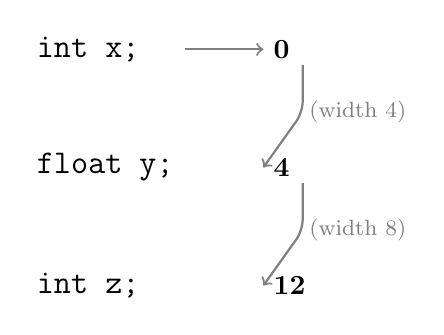
\begin{tikzpicture}[scale=1]
        % Testo del codice
        \node[anchor=west, font=\large] (L1) at (0, 3) {\texttt{int x;}};
        \node[anchor=west, font=\large] (L2) at (0, 1.5) {\texttt{float y;}};
        \node[anchor=west, font=\large] (L3) at (0, 0) {\texttt{int z;}};
    
        % Frecce e valori offset
        % Riga 1
        \draw[->, gray, thick] (2, 3) -- (3, 3) node[right, black] {\textbf{0}};
        
        % Freccia da riga 1 a riga 2 (somma width)
        \draw[->, gray, thick, rounded corners] (3.5, 2.8) -- (3.5, 2.2) -- (3, 1.5) node[right, black] {\textbf{4}}; 
        \node[text=gray, font=\footnotesize] at (4.2, 2.2) {(width 4)};
    
        % Freccia da riga 2 a riga 3
        \draw[->, gray, thick, rounded corners] (3.5, 1.3) -- (3.5, 0.7) -- (3, 0) node[right, black] {\textbf{12}};
        \node[text=gray, font=\footnotesize] at (4.2, 0.7) {(width 8)};
    
    \end{tikzpicture}
    \end{center}

\subsection{SEQUENZE DI DICHIARAZIONI}

Prima che la prima delle dichiarazioni sia analizzata, il valore della variabile \textit{offset} viene inizializzato a 0. Ogni volta che viene individuato un nuovo nome, esso viene inserito nella tabella dei simboli con l'offset corrente, incrementato poi della larghezza del tipo.

\begin{align*}
P &\to \quad \{ offset = 0; \} \\
  &\quad \ \ D \\[1em]
D &\to T \ \mathbf{id} ; \quad \{ top.put(\mathbf{id}.lexeme, T.type, offset); \\
  &\quad \quad \quad \quad \quad \quad offset = offset + T.width; \} \\
  &\quad \ \ D_1 \\[1em]
D &\to \epsilon
\end{align*}

\vspace{0.5cm}
\noindent \textbf{Esempio :}

\begin{center}
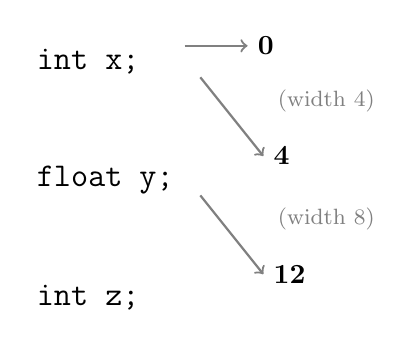
\begin{tikzpicture}[x=1cm, y=1cm]
    % Codice
    \node[anchor=west, font=\large] at (0, 3) {\texttt{int x;}};
    \node[anchor=west, font=\large] at (0, 1.5) {\texttt{float y;}};
    \node[anchor=west, font=\large] at (0, 0) {\texttt{int z;}};

    % Frecce e valori offset
    \draw[->, gray, thick] (2, 3.2) -- (2.8, 3.2) node[right, black] {\textbf{0}};
    
    \draw[->, gray, thick] (2.2, 2.8) -- (3, 1.8) node[right, black] {\textbf{4}}; 
    \node[text=gray, font=\footnotesize] at (3.8, 2.5) {(width 4)};

    \draw[->, gray, thick] (2.2, 1.3) -- (3, 0.3) node[right, black] {\textbf{12}};
    \node[text=gray, font=\footnotesize] at (3.8, 1) {(width 8)};

\end{tikzpicture}
\end{center}

\subsection{CAMPI NEI RECORD E NELLE CLASSI}

La produzione che ci interessa è:
$$ T \to \mathbf{record} \ '\{' \ D \ '\}' $$

Un approccio simile a quello delle dichiarazioni può essere esteso ai tipi e agli indirizzi relativi ai campi, a patto che siano soddisfatte due condizioni:
\begin{itemize}
    \item I nomi dei campi di un record devono essere tutti distinti (cioè ogni nome può apparire una sola volta nelle dichiarazioni generate da $D$).
    \item L'indirizzo relativo è dato rispetto all'indirizzo di base dello specifico record.
\end{itemize}

Per comodità ogni tipo record utilizzerà una tabella dei simboli locale per memorizzare le informazioni relative a tipo e indirizzo relativo dei suoi campi. Un tipo record ha la
forma record (t) in cui record() è il costruttore di tipo e t è un oggetto che rappresenta
la tabella dei simboli contenente tutte le informazioni relative ai campi del record.

\vspace{0.3cm}
\noindent \textbf{Esempio :}
L'uso di un nome $x$ per indicare un campo di un record non entra in conflitto con altri usi dello stesso nome al di fuori del record.

\begin{verbatim}
    float x;
    record { float x; float y; } p;
    record { int tag; float x; float y; } q;
\end{verbatim}


%lezione 1 dicembre
\vspace{1 cm}
\subsection{Traduzione delle Espressioni}

La definizione guidata dalla sintassi (SDT) mostrata nella tabella seguente costruisce il codice a tre indirizzi di un'istruzione di assegnamento $S$ facendo ricorso all'attributo \emph{code} di $S$ e agli attributi \emph{code} e \emph{addr} dell'espressione denotata da $E$.

Gli attributi $S.code$ ed $E.code$ indicano il codice a tre indirizzi relativo rispettivamente a $S$ ed $E$. L'attributo $E.addr$, invece, indica l'indirizzo della locazione di memoria che conterrà il valore di $E$. Si tenga presente che un indirizzo può essere un nome, una costante oppure una variabile temporanea generata dal compilatore.

\begin{table}[h]
    \centering
    \renewcommand{\arraystretch}{1.5}
    \begin{tabular}{|l|p{10cm}|}
        \hline
        \textbf{Produzione} & \textbf{Regole Semantiche} \\
        \hline
        $S \rightarrow \textbf{id} = E;$ & $S.code = E.code \parallel gen(top.get(\textbf{id}.lexeme) \text{ '=' } E.addr)$ \\
        \hline
        $E \rightarrow E_1 + E_2$ & $E.addr = \text{new Temp}()$ \\
                                  & $E.code = E_1.code \parallel E_2.code \parallel gen(E.addr \text{ '=' } E_1.addr \text{ '+' } E_2.addr)$ \\
        \hline
        $E \rightarrow - E_1$ & $E.addr = \text{new Temp}()$ \\
                              & $E.code = E_1.code \parallel gen(E.addr \text{ '=' } \text{'minus' } E_1.addr)$ \\
        \hline
        $E \rightarrow ( E_1 )$ & $E.addr = E_1.addr$ \\
                                & $E.code = E_1.code$ \\
        \hline
        $E \rightarrow \textbf{id}$ & $E.addr = top.get(\textbf{id}.lexeme)$ \\
                                    & $E.code = ""$ (stringa vuota) \\
        \hline
    \end{tabular}
    \caption{SDT per la generazione di codice a tre indirizzi per le espressioni.}
\end{table}

\subsubsection*{Analisi delle Regole Semantiche}

Si consideri l'ultima produzione $E \rightarrow \textbf{id}$ della Figura. Quando un'espressione coincide con un singolo identificatore $x$, $x$ stesso contiene il valore dell'espressione. Per questa ragione la regola semantica associata a tale produzione assegna all'attributo $E.addr$ il puntatore all'elemento della tabella dei simboli che si riferisce alla specifica occorrenza di \textbf{id}.
Se $top$ indica la tabella dei simboli corrente, la funzione $top.get()$ restituisce l'elemento della tabella dei simboli individuato in base alla stringa $\textbf{id}.lexeme$ relativa all'istanza di \textbf{id} in esame. All'attributo $E.code$ viene invece assegnata la stringa vuota.

Quando invece si considera la produzione $E \rightarrow ( E_1 )$, la traduzione di $E$ coincide con quella della sottoespressione $E_1$, pertanto $E.addr$ prende il valore di $E_1.addr$ ed $E.code$ prende il valore di $E_1.code$.

I due operatori di somma (+) e di negazione (cioè il $-$ unario) sono rappresentativi della maggioranza degli operatori nei comuni linguaggi di programmazione. Le regole semantiche associate alla produzione $E \rightarrow E_1 + E_2$ generano il codice per calcolare il valore di $E$ a partire dai valori di $E_1$ ed $E_2$. Il risultato è assegnato a una nuova variabile temporanea generata dal compilatore.
Se il valore di $E_1$ è assegnato a $E_1.addr$ ed $E_2$ a $E_2.addr$, allora $E_1 + E_2$ viene tradotto come $t = E_1.addr + E_2.addr$, in cui $t$ è un nuovo nome temporaneo.

Infine, il valore di $t$ viene assegnato a $E.addr$. Si noti che esecuzioni successive dell'istruzione \texttt{new Temp()} producono una sequenza di nomi temporanei $t_1, t_2, \dots$ tutti distinti.

Per comodità usiamo la notazione $gen(x \text{ '=' } y \text{ '+' } z)$ per indicare l'istruzione a tre indirizzi $x = y + z$. Eventuali espressioni che dovessero apparire al posto delle variabili $x, y$ e $z$ sarebbero valutate prima di essere passate alla funzione $gen()$; le stringhe tra apici, invece, sono interpretate letteralmente.
Altre istruzioni a tre indirizzi sono costruite in modo simile, applicando la funzione $gen()$ a una combinazione di espressioni e stringhe costanti.

Le regole di traduzione associate alla produzione $E \rightarrow E_1 + E_2$ costruiscono $E.code$ concatenando $E_1.code$, $E_2.code$ e un'istruzione che somma i valori di $E_1$ ed $E_2$. Tale istruzione assegna il risultato della somma a un nuovo nome temporaneo associato a $E$ e indicato da $E.addr$.

La traduzione della produzione $E \rightarrow - E_1$ è simile. Le regole semantiche dapprima creano un nuovo nome temporaneo per $E$, quindi generano un'istruzione che esegue l'operazione di negazione (meno unario).

Infine, la produzione $S \rightarrow \textbf{id} = E;$ genera le istruzioni che assegnano il valore dell'espressione $E$ all'identificatore \textbf{id}. Le regole semantiche associate a questa produzione utilizzano la funzione $top.get()$ per determinare l'indirizzo dell'identificatore rappresentato da \textbf{id}, esattamente come già visto per la produzione $E \rightarrow \textbf{id}$.
Il valore dell'attributo $S.code$ consiste delle istruzioni per calcolare il valore di $E$ e assegnarlo all'indirizzo indicato da $E.addr$, seguite da un'assegnamento all'indirizzo restituito dalla funzione $top.get(\textbf{id}.lexeme)$ e relativo alla specifica istanza di \textbf{id} in esame.

\subsubsection*{Esempio}
L'assegnamento $a = b + -c$ viene tradotto visualizzando l'albero sintattico annotato qui sotto:

\begin{center}
\begin{forest}
    for tree={
        font=\large,
        s sep=1.5cm,
        l sep=1.2cm,
        edge=thick,
        align=center 
    }
    [{=}, label={right:{\small (3) $S \to \textbf{id} = E$}}
        [\textbf{a}]
        [{+}, label={right:{\small (2) $E \to E_1 + E_2$}}
            [\textbf{b}]
            [{-}, label={right:{\small (1) $E \to - E_1$}}
                [\textbf{c}]
            ]
        ]
    ]
\end{forest}
\end{center}
\vspace{2 cm}
La sequenza di codice a tre indirizzi generata è:
\begin{lstlisting}
t1 = minus c
t2 = b + t1
a = t2
\end{lstlisting}
\subsubsection{Traduzione incrementale}

Come sappiamo, gli attributi \texttt{code} possono diventare stringhe di notevoli dimensioni. Per questa ragione, è preferibile generare le istruzioni in modo incrementale. Invece di costruire $E.code$, la funzione $gen()$ scrive direttamente l'istruzione nel file di output.

Ecco lo schema di traduzione modificato:

\begin{table}[H]
    \centering
    \renewcommand{\arraystretch}{1.5}
    \begin{tabular}{|l|p{10cm}|}
        \hline
        \textbf{Produzione} & \textbf{Azioni Semantiche (Incrementali)} \\
        \hline
        $S \rightarrow \textbf{id} = E;$ & $gen(top.get(\textbf{id}.lexeme) \text{ '=' } E.addr);$ \\
        \hline
        $E \rightarrow E_1 + E_2$ & $E.addr = \text{new Temp}();$ \\
                                  & $gen(E.addr \text{ '=' } E_1.addr \text{ '+' } E_2.addr);$ \\
        \hline
        $E \rightarrow - E_1$ & $E.addr = \text{new Temp}();$ \\
                              & $gen(E.addr \text{ '=' } \text{'minus' } E_1.addr);$ \\
        \hline
        $E \rightarrow ( E_1 )$ & $E.addr = E_1.addr;$ \\
        \hline
        $E \rightarrow \textbf{id}$ & $E.addr = top.get(\textbf{id}.lexeme);$ \\
        \hline
    \end{tabular}
    \caption{SDT per la costruzione incrementale del codice a tre indirizzi delle espressioni.}
\end{table}

\textbf{Costruzione dell'Albero Sintattico:}
Questo approccio può essere utilizzato anche per costruire alberi sintattici. In tal caso, l'azione semantica $ E \rightarrow E_1 + E_2 $ creerebbe un nuovo nodo, utilizzando il costruttore Node():
$$ E \rightarrow E_1 + E_2 \quad \{ E.addr = \text{new Node}('+', E_1.addr, E_2.addr); \} $$
Qui $addr$ rappresenta l'indirizzo (puntatore) del nodo creato.

Di seguito le regole semantiche specifiche per la creazione dei nodi (trascritte dagli appunti):

\begin{itemize}
    \item \textbf{Produzione} $E \to \textbf{id}$ \\
    Si crea una foglia che contiene il riferimento alla voce nella tabella dei simboli:
    $$ \{ E.addr = \text{new Leaf}(\textbf{id}, \textbf{id}.entry); \} $$

    \item \textbf{Produzione} $E \to - E_1$ \\
    Si crea un nodo per l'operatore unario \texttt{minus} (che ha un solo figlio):
    $$ \{ E.addr = \text{new Node}(\text{minus}, E_1.addr); \} $$

    \item \textbf{Produzione} $S \to \textbf{id} = E$ \\
    Si crea prima una foglia per l'identificatore a sinistra, e poi il nodo di assegnamento che collega l'identificatore all'espressione:
    \begin{align*}
        \{ \quad & addr = \text{new Leaf}(\textbf{id}, \textbf{id}.entry); \\
                 & S.addr = \text{new Node}('=', addr, E.addr); \quad \}
    \end{align*}
\end{itemize}

\subsubsection{Indirizzamento degli elementi di un array}

Per accedere agli elementi di un array, è necessario calcolare l'offset rispetto all'indirizzo di base se questi sono memorizzati in blocchi contigui.

\subsubsection*{Calcolo degli Indirizzi}

\subsubsection*{Array Monodimensionale}
Se gli indici partono da 0, l'indirizzo dell'$i$-esimo elemento è:
\begin{equation}
    base + i \times w
\end{equation}
dove $w$ è la larghezza (dimensione in byte) di ogni elemento, e $base$ è l'indirzzo relativo dell'inizio della zona di memoria riservata all'array.

\textbf{Generalizzazione (indice non zero):}
Se gli elementi sono numerati da un indice $low$ a $high$, l'indirizzo diventa:
\begin{equation}
    base + (i - low) \times w
\end{equation}
Questa formula può essere riscritta per pre-calcolare la parte costante a compile-time:
$$ i \times w + (base - low \times w) $$
Dove $(base - low \times w) = c$ viene calcolato una sola volta e salvato nella tabella dei simboli.

\subsubsection*{Array Multidimensionali}
Per un array a due dimensioni ($n_1 \times n_2$) memorizzato per righe, l'indirizzo dell'elemento $A[i_1, i_2]$ è:
\begin{equation}
    base + (i_1 \times n_2 + i_2) \times w
\end{equation}
In $k$ dimensioni, la formula generalizzata è:
\begin{equation}
    (\dots((i_1 \times n_2 + i_2) \times n_3 + i_3) \dots ) \times n_k + i_k ) \times w
\end{equation}

\subsubsection*{Memorizzazione in Memoria}

Un array bidimensionale può essere memorizzato per righe (come in C e Java) o per colonne.

\begin{figure}[h]
    \centering
    \begin{tikzpicture}[
        node distance=0pt,
        start chain=1 going below,
        start chain=2 going below,
        box/.style={draw, minimum width=2.5cm, minimum height=0.8cm, outer sep=0pt}
    ]
        % Colonna sinistra: Per righe
        \node [on chain=1] (label1) {\textbf{(a) Per righe}};
        \node [on chain=1, box] (r1) {$A[0,0]$};
        \node [on chain=1, box] (r2) {$A[0,1]$};
        \node [on chain=1, box] (r3) {$A[0,2]$};
        \node [on chain=1, box] (r4) {$A[1,0]$};
        \node [on chain=1, box] (r5) {$A[1,1]$};
        \node [on chain=1, box] (r6) {$A[1,2]$};

        % Parentesi graffe per righe
        \draw [decorate,decoration={brace,amplitude=5pt}]
        ($(r1.north east)+(0.2,0)$) -- ($(r3.south east)+(0.2,0)$) node [midway, right=6pt] {Prima riga};
        
        \draw [decorate,decoration={brace,amplitude=5pt}]
        ($(r4.north east)+(0.2,0)$) -- ($(r6.south east)+(0.2,0)$) node [midway, right=6pt] {Seconda riga};

        % Colonna destra: Per colonne (posizionata a destra)
        \node [on chain=2, right=5cm of label1] (label2) {\textbf{(b) Per colonne}};
        \node [on chain=2, box] (c1) {$A[0,0]$};
        \node [on chain=2, box] (c2) {$A[1,0]$};
        \node [on chain=2, box] (c3) {$A[0,1]$};
        \node [on chain=2, box] (c4) {$A[1,1]$};
        \node [on chain=2, box] (c5) {$A[0,2]$};
        \node [on chain=2, box] (c6) {$A[1,2]$};

        % Parentesi graffe per colonne
        \draw [decorate,decoration={brace,amplitude=5pt}]
        ($(c1.north east)+(0.2,0)$) -- ($(c2.south east)+(0.2,0)$) node [midway, right=6pt] {Prima col.};
        
        \draw [decorate,decoration={brace,amplitude=5pt}]
        ($(c3.north east)+(0.2,0)$) -- ($(c4.south east)+(0.2,0)$) node [midway, right=6pt] {Seconda col.};
        
        \draw [decorate,decoration={brace,amplitude=5pt}]
        ($(c5.north east)+(0.2,0)$) -- ($(c6.south east)+(0.2,0)$) node [midway, right=6pt] {Terza col.};

    \end{tikzpicture}
    \caption{Organizzazione della memoria per un array $2 \times 3$.}
\end{figure}

Nell'organizzazione per \textbf{righe}, l'indice più a destra cambia più rapidamente. In quella per \textbf{colonne}, cambia più rapidamente l'indice a sinistra.

\subsubsection{Traduzione dei Riferimenti agli Array}
Il problema principale nella generazione del codice per i riferimenti agli elementi di un array è correlare i calcoli dell'indirizzo del paragrafo precedente alla grammatica corrispondente.
La grammatica per i riferimenti agli array usa il non-terminale $L$ per gestire sequenze di indici:
$$ L \rightarrow L[E] \mid \textbf{id}[E] $$
Assumiamo che l'indice del primo elemento sia 0 e usiamo il calcolo basato sulle larghezze (Eq. 4).

\subsubsection*{Attributi per L}
Il non-terminale $L$ ha tre attributi sintetizzati:
\begin{enumerate}
    \item \textbf{L.addr}: Un indirizzo temporaneo utilizzato per il calcolo dello spiazzamento (la somma dei termini $i_j \times w_j$).
    \item \textbf{L.array}: Un puntatore all'elemento della tabella dei simboli relativo al nome dell'array.
    \item \textbf{L.type}: Il tipo del sotto-array generato da $L$. Usiamo \texttt{t.width} per la larghezza e \texttt{t.elem} per il tipo degli elementi.
\end{enumerate}

\subsubsection*{Schema di Traduzione (SDT)}
Lo schema di traduzione genera codice a tre indirizzi per espressioni con array:

\begin{table}[H]
    \centering
    \renewcommand{\arraystretch}{1.5}
    \begin{tabular}{|l|p{10cm}|}
        \hline
        \textbf{Produzione} & \textbf{Azioni Semantiche} \\
        \hline
        $S \rightarrow \textbf{id} = E;$ & $gen(top.get(\textbf{id}.lexeme) \text{ '=' } E.addr);$ \\
        \hline
        $S \rightarrow L = E;$ & $gen(L.array.base \text{ '[' } L.addr \text{ ']' '=' } E.addr);$ \\
        \hline
        $E \rightarrow E_1 + E_2$ & $E.addr = \text{new Temp}();$ \\
                                  & $gen(E.addr \text{ '=' } E_1.addr \text{ '+' } E_2.addr);$ \\
        \hline
        $E \rightarrow \textbf{id}$ & $E.addr = top.get(\textbf{id}.lexeme);$ \\
        \hline
        $E \rightarrow L$ & $E.addr = \text{new Temp}();$ \\
                          & $gen(E.addr \text{ '=' } L.array.base \text{ '[' } L.addr \text{ ']' } );$ \\
        \hline
        $L \rightarrow \textbf{id}[E]$ & $L.array = top.get(\textbf{id}.lexeme);$ \\
                                       & $L.type = L.array.type.elem;$ \\
                                       & $L.addr = \text{new Temp}();$ \\
                                       & $gen(L.addr \text{ '=' } E.addr \text{ '*' } L.type.width);$ \\
        \hline
        $L \rightarrow L_1[E]$ & $L.array = L_1.array;$ \\
                               & $L.type = L_1.type.elem;$ \\
                               & $t = \text{new Temp}();$ \\
                               & $L.addr = \text{new Temp}();$ \\
                               & $gen(t \text{ '=' } E.addr \text{ '*' } L.type.width);$ \\
                               & $gen(L.addr \text{ '=' } L_1.addr \text{ '+' } t);$ \\
        \hline
    \end{tabular}
    \caption{Azioni semantiche per la traduzione dei riferimenti ad array.}
\end{table}

\subsubsection{Esempio: Albero Annotato}
Sia $a$ un array di interi di dimensione $2 \times 3$ e siano $c, i, j$ variabili intere.
\begin{itemize}
    \item Il tipo di $a$ è $array(2, array(3, integer))$, larghezza $2 \times 3 \times 4 = 24$.
    \item Il tipo di $a[i]$ è $array(3, integer)$, larghezza $12$.
    \item Il tipo di $a[i][j]$ è $integer$, larghezza $4$.
\end{itemize}

Consideriamo l'espressione:
$$ c + a[i][j] $$

\textbf{Codice a tre indirizzi generato:}
\begin{lstlisting}
t1 = i * 12
t2 = j * 4
t3 = t1 + t2
t4 = a[t3]
t5 = c + t4
\end{lstlisting}

\textbf{Albero di parsing annotato:}

\begin{center}
    \begin{forest}
        for tree={
            font=\small,
            s sep=0.5cm,    % Spazio orizzontale ridotto per farci stare tutto
            l sep=1.2cm,    % Spazio verticale
            edge=->,
            align=center    % <--- FONDAMENTALE: risolve l'errore "Not allowed in LR mode"
        }
        [{$E.addr = t_5$}, name=root
            [{$E.addr = c$}
                [\textbf{c}]
            ]
            [{+} ]
            [{$E.addr = t_4$}
                [{$L.array = a$ \\ $L.type = \text{integer}$ \\ $L.addr = t_3$}
                    [{$L.array = a$ \\ $L.type = \text{array}(3, \text{int})$ \\ $L.addr = t_1$}
                        [{$a.type =
                        array(2,array(3,integer))$}]
                        [{[}]
                        [{$E.addr = i$} [\textbf{i}] ]
                        [{]}]
                    ]
                    [{[}]
                    [{$E.addr = j$} [\textbf{j}] ]
                    [{]}]
                ]
            ]
        ]
    \end{forest}
    \end{center}

    

%lezione 10 dicembre
\subsection{Controllo dei Tipi}

Il controllo dei tipi (Type Checking) consiste nel verificare che il programma rispetti le regole del sistema di tipi del linguaggio (Type System). Il compilatore deve:
\begin{enumerate}
    \item Assegnare un'espressione di tipo a ogni componente del programma.
    \item Procedere a verificare che tali espressioni siano conformi a un insieme di regole logiche.
\end{enumerate}

Un linguaggio è \textbf{fortemente tipizzato} se il compilatore garantisce che i programmi accettati verranno eseguiti senza errori di tipo.

\subsubsection{Regole per il Controllo dei Tipi}

Il controllo può assumere due forme: \textit{sintesi} e \textit{inferenza}.

\subsubsection*{Sintesi dei Tipi}
Prevede la costruzione del tipo di un'espressione a partire dal tipo delle sue sottoespressioni. I nomi devono essere dichiarati prima dell'uso.
Una tipica regola di sintesi è :
$$
\textbf{if } f \text{ è di tipo } s \to t \textbf{ and } x \text{ è di tipo } s, 
$$
$$
\textbf{ then } f(x) \text{ è di tipo } t
$$
Questa regola può essere applicata anche a operatori come la somma ($E_1 + E_2$), interpretandoli come funzioni $add(E_1, E_2)$.

\subsubsection*{Inferenza dei Tipi}
Determina il tipo di un costrutto del linguaggio in base al modo in cui viene utilizzato.
Esempio: se abbiamo una funzione $null(x)$ che verifica se una lista è vuota, dall'espressione $null(x)$ inferiamo che $x$ deve essere una lista, anche se non conosciamo il tipo degli elementi.

Useremo le lettere greche ($\alpha, \beta$) per indicare tipi ignoti. La regola tipica è la seguente:
$$
    \textbf{if } f(x) \text{ è un'espressione, }
$$
$$
    \textbf{then} \text{ per qualche } \alpha \text{ e } \beta \text{, f è di tipo } \alpha \to \beta \textbf{ and } x \text{ è di tipo } \alpha
$$

\textbf{Esempio: Statement If}
Possiamo interpretare il costrutto \texttt{if(E) S;} come l'applicazione di una funzione che richiede un booleano e uno statement (tipo \textit{void}) e restituisce \textit{void}:
$$ if: boolean \times void \to void $$

\subsubsection{Conversioni di Tipo}

Consideriamo un'espressione aritmetica del tipo $x + i$, in cui $x$ è di tipo \texttt{float} e $i$ è di tipo \texttt{integer}.
Poiché la loro rappresentazione interna è diversa nei calcolatori, e le operazioni su di essi richiedono istruzioni macchina differenti, il compilatore deve gestire la situazione in modo che entrambi gli operandi abbiano lo stesso tipo al momento dell'esecuzione della somma.

Supponiamo che i valori interi debbano essere convertiti in valori floating-point quando necessario, mediante l'operatore unario \texttt{(float)}.
Ad esempio, nel codice dell'espressione $2 * 3.14$, il valore intero 2 viene convertito in virgola mobile:
\begin{lstlisting}[language=C]
t1 = (float) 2
t2 = t1 * 3.14
\end{lstlisting}

\paragraph{Tipologie di Conversione}
Le conversioni possono essere classificate in base a chi le effettua:
\begin{itemize}
    \item \textbf{Implicita (Coercizione):} La conversione avviene automaticamente a cura del compilatore. Si limitano solitamente a promozioni che garantiscono la consistenza dell'informazione.
    \item \textbf{Esplicita (Cast):} Il programmatore scrive istruzioni apposite per forzare la conversione.
\end{itemize}

\subsubsection*{Regole di Conversione in Java}

Le regole variano da linguaggio a linguaggio. In Java si distinguono due casi principali:

\begin{enumerate}
    \item \textbf{Conversioni con ampliamento (Widening):} Anche dette \textit{promozioni}. Hanno lo scopo di preservare l'informazione intatta trasformando un tipo in uno più grande (gerarchicamente superiore).
    \item \textbf{Conversioni con restrizione (Narrowing):} Anche dette \textit{demozioni}. Possono portare a una perdita di informazione (es. troncamento dei decimali).
\end{enumerate}

Le regole sono descritte dai grafici seguenti. Una conversione da un tipo $s$ a un tipo $t$ è lecita se e solo se esiste un arco da $s$ a $t$.

\begin{figure}[H]
    \centering
    \begin{tikzpicture}[node distance=1cm, auto, >=latex]
        % Stile dei nodi
        \tikzstyle{type} = [draw=none, fill=none]
        
        % --- GRAFO (a) Promozioni (Widening) ---
        \node[type] (double) {double};
        \node[type, below=0.6cm of double] (float) {float};
        \node[type, below=0.6cm of float] (long) {long};
        \node[type, below=0.6cm of long] (int) {int};
        \node[type, below left=0.8cm of int] (short) {short};
        \node[type, below left=0.6cm of short] (byte) {byte};
        \node[type, below right=0.8cm of int] (char) {char};
        
        \draw[->] (float) -- (double);
        \draw[->] (long) -- (float);
        \draw[->] (int) -- (long);
        \draw[->] (short) -- (int);
        \draw[->] (byte) -- (short);
        \draw[->] (char) -- (int);
        
        \node[below=6cm of double] {(a) Promozioni};

        % --- GRAFO (b) Demozioni (Narrowing) ---
        \node[type, right=4cm of double] (double2) {double};
        \node[type, below=0.6cm of double2] (float2) {float};
        \node[type, below=0.6cm of float2] (long2) {long};
        \node[type, below=0.6cm of long2] (int2) {int};
        
        \node[type, below=0.6cm of int2] (short2) {short};
        \node[type, left=0.8cm of short2] (char2) {char}; 
        \node[type, right=0.8cm of short2] (byte2) {byte}; 

        \draw[->] (double2) -- (float2);
        \draw[->] (float2) -- (long2);
        \draw[->] (long2) -- (int2);
        \draw[->] (int2) -- (short2);
        \draw[->] (short2) -- (byte2);
        \draw[->] (int2) -- (byte2);
        
        % Conversioni incrociate specifiche (Narrowing)
        \draw[->] (int2) -- (char2);
        
        % Relazione reciproca char <-> short
        \draw[<->] (char2) -- (short2); 
        
        % Relazione reciproca char <-> byte
        \draw[<->] (char2) to[bend right=45] (byte2); 

        \node[below=1.4cm of short2] {(b) Demozioni};
        
    \end{tikzpicture}
    \caption{Gerarchia delle conversioni tra tipi primitivi in Java. Si noti che \texttt{char}, \texttt{short} e \texttt{byte} sono convertibili l'uno nell'altro nelle demozioni.}
\end{figure}

\subsubsection*{Generazione del Codice Semantico}

L'azione semantica per il controllo di tipo della produzione $E \to E_1 + E_2$ utilizza due funzioni ausiliarie fondamentali:

\begin{enumerate}
    \item $\textbf{max}(t_1, t_2)$: Prende come argomenti due tipi $t_1$ e $t_2$ e restituisce il maggiore dei due secondo la gerarchia di promozione (widening).
    \item $\textbf{widen}(a, t, w)$: Genera la conversione di tipo necessaria per promuovere un indirizzo $a$ di tipo $t$ in un valore di tipo $w$.
\end{enumerate}

\textbf{Funzionamento di \texttt{widen}:}
Se $t$ e $w$ rappresentano lo stesso tipo, la funzione restituisce $a$ stesso. Altrimenti, genera un'istruzione che esegue la conversione, salva il risultato in una variabile temporanea \texttt{temp} e restituisce \texttt{temp}.

Ecco lo pseudocodice, assumendo che gli unici tipi disponibili siano \texttt{integer} e \texttt{float}:

\begin{lstlisting}
Addr widen(Addr a, Type t, Type w) {
    if (t == w) return a;
    else if (t == integer and w == float) {
        temp = new Temp();
        gen(temp '=' '(float)' a);
        return temp;
    }
    else error;
}
\end{lstlisting}

\paragraph{Schema di Traduzione (SDT)}
L'uso di queste funzioni permette di generalizzare lo schema di traduzione, evitando una lunga serie di controlli condizionali annidati (es. "se $E_1$ è int ed $E_2$ è float...").

Il nuovo schema per la somma diventa:

\begin{lstlisting}
E -> E1 + E2  {
    // 1. Determina il tipo risultato (il "massimo" tra i due)
    E.type = max(E1.type, E2.type);
    
    // 2. Converte (se necessario) entrambi gli operandi al tipo risultato
    a1 = widen(E1.addr, E1.type, E.type);
    a2 = widen(E2.addr, E2.type, E.type);
    
    // 3. Genera il codice per la somma usando gli indirizzi (eventualmente) convertiti
    E.addr = new Temp();
    gen(E.addr '=' a1 '+' a2);
}
\end{lstlisting}

\subsubsection{Sovraccarico delle Funzioni (Overloading)}

Il sovraccarico (o overloading) si verifica quando uno stesso simbolo ha significati diversi. Il problema principale consiste nel \textbf{disambiguare} quale versione del simbolo utilizzare, basandosi sul contesto.

La scelta dell'interpretazione corretta avviene osservando:
\begin{itemize}
    \item Gli \textbf{argomenti} forniti in una chiamata di funzione.
    \item Le \textbf{operazioni} applicate al risultato (o a una variabile).
\end{itemize}

\paragraph{Assunzione}
Per semplificare il problema, assumiamo che il sovraccaricamento sia risolvibile analizzando \textbf{esclusivamente} i tipi degli argomenti di una funzione.

Una possibile regola per la sintesi del tipo di funzioni sovraccaricate è la seguente:

\begin{gather*}
    \textbf{if } f \text{ può essere di tipo } s_i \to t_i, \text{ per } 1 \le i \le n, \text{ con } s_i \neq s_j \text{ per } i \neq j \\
    \textbf{and } x \text{ è di tipo } s_k, \text{ per qualche valore di } k \text{ tale che } 1 \le k \le n \\
    \textbf{then } \text{l'espressione } f(x) \text{ è di tipo } t_k
\end{gather*}

\paragraph{Risoluzione efficiente (tramite metodo del valore numerico)}
Per risolvere efficientemente il problema del sovraccaricamento, si può assegnare un indice intero (valore numerico) a ogni nodo di un DAG che rappresenta l'espressione.
La \textbf{firma} di una funzione consiste nel nome della funzione e nel tipo dei suoi argomenti. L'ipotesi di poter risolvere il sovraccaricamento sulla base dei soli argomenti equivale a dire che possiamo risolverlo in base alla firma.

\textit{Nota:} Non sempre l'analisi dei soli argomenti è sufficiente. 





%lezione 11 dicembre
\subsubsection{Inferenza del Tipo}

L'inferenza del tipo determina il tipo di un costrutto del linguaggio in base al modo in cui esso è utilizzato. L'inferenza di tipo assicura che i nomi siano usati in modo consistente.

Il termine \textbf{polimorfico} indica in generale un qualsiasi frammento di codice che possa essere eseguito con argomenti di diversi tipi. In questo paragrafo considereremo il \textbf{polimorfismo parametrico}, caratterizzato da parametri o variabili di tipo.

Una tipica regola per l'inferenza di tipo ha la forma seguente:
\begin{quote}
    \textbf{if} $f(x)$ è un'espressione,\\
    \textbf{then} per qualche $\alpha$ e $\beta$, $f$ è di tipo $\alpha \to \beta$ \textbf{and} $x$ è di tipo $\alpha$.
\end{quote}
\subsubsection*{Sostituzioni, Istanze e Unificazione}

Se $t$ è un'espressione di tipo e $S$ una sostituzione (cioè un mapping tra variabili di tipo ed espressioni di tipo), la scrittura $S(t)$ indica il risultato che si ottiene sostituendo tutte le occorrenze di ogni variabile di tipo $\alpha$ con $S(\alpha)$.

Chiamiamo $S(t)$ una \textbf{istanza} di $t$.
Per esempio, $list(integer)$ è un'istanza di $list(\alpha)$, poiché è il risultato della sostituzione di $\alpha$ con $integer$, così come $integer \to integer$, mentre $integer \to float$ non è un'istanza di $\alpha \to \alpha$ poiché una sostituzione prevede che ogni occorrenza di una data variabile di tipo sia rimpiazzata dalla stessa espressione di tipi.

Diciamo che la sostituzione $S$ è un \textbf{unificatore} delle espressioni di tipo $t_1$ e $t_2$ se risulta $S(t_1) = S(t_2)$ (ce ne può essere più di uno).
Diciamo inoltre che $S$ è l'\textit{unificatore più generale} di $t_1$ e $t_2$ se per qualsiasi altro unificatore $S'$ di $t_1$ e $t_2$, $S'$ impone vincoli più stringenti di quanto non faccia $S$.

\subsubsection*{Algoritmo di Inferenza di Tipo per Funzioni Polimorfiche}

\textbf{Input:} Un programma consistente in una sequenza di definizioni di funzione seguita da un'espressione da valutare.

\noindent \textbf{Output:} Tipi inferiti dei nomi che appaiono nel programma.

\noindent \textbf{Metodo:}
Per semplicità tratteremo solamente le funzioni unarie. Il tipo di una funzione binaria $f(x_1, x_2)$ può essere descritto dall'espressione di tipo $s_1 \text{ x } s_2 \to t$ in cui $s_1$ e $s_2$ sono i tipi di $x_1$ e $x_2$ rispettivamente e t è il tipo del risultato $f(x_1, x_2)$. Una
espressione come $f(a, b)$ può essere controllata confrontando $a$ con $s_1$ e $b$ con $s_2$.
L'idea di base consiste nello scorrere le definizioni di funzione e l'espressione nel programma d'ingresso e nell'utilizzare il tipo già inferito di una funzione ogniqualvolta questa appare in un'espressione successiva.

\begin{itemize}
    \item Per una definizione di funzione della forma $\textbf{fun } id_1(id_2) = E$, si creano due nuove variabili di tipo $\alpha$ e $\beta$. Si associa alla funzione $id_1$ il tipo $\alpha \to \beta$ e al parametro $id_2$ il tipo $\alpha$. Quindi si inferisce un'espressione di tipo per $E$. Supponiamo che, dopo l'inferenza, $\alpha$ denoti il tipo $s$ e $\beta$ il tipo t. Ne risulta che il tipo inferito per la funzione $id_1$ è $s \to t$. Ciò fatto, si legano mediante il quantificatore $\forall$ tutte le variabili rimaste non vincolate.
    \item Per l'applicazione di una funzione $E_1(E_2)$, si inferiscono i tipi di $E_1$ ed $E_2$. Dato che $E_1$ è usato come funzione, il suo tipo deve essere della forma $s \to s'$. Si cerca di unificare il tipo di $E_1$ con $\beta \to \gamma$ (dove $\beta$ è il tipo di $E_2$). Sia $t$ il tipo inferito di $E_2$. Si cerca di unificare $s$ e $t$: se il tentativo fallisce si ha un errore di tipo, altrimenti il tipo inferito di $E_1(E_2)$ è $s'$. (Es: $S \to \alpha \to \alpha$ e $S \to integer$, allora $\alpha \to integer$).
    \item Per ogni occorrenza di una funzione polimorfica, si sostituisce ogni variabile legata dal quantificatore $\forall$ con una nuova variabile e si rimuove il quantificatore.
    \item Per un nome che si incontra per la prima volta, si introduce una nuova variabile di tipo.
\end{itemize}

\subsubsection*{Esempio: Inferenza su Funzione Polimorfica}

Consideriamo il programma in linguaggio ML che definisce la funzione $length()$.
\textbf{fun} introduce la definizione di una funzione; $null()$ verifica se una lista è vuota, mentre la funzione predefinita $tl()$ (\textit{tail}) restituisce ciò che rimane di una lista dopo aver rimosso il primo elemento.

$$ \textbf{fun } length(x) = \textbf{if } null(x) \textbf{ then } 0 \textbf{ else } length(tl(x)) + 1 $$

\subsubsection*{Analisi dell'Albero Sintattico}

\begin{figure}[h]
    \centering
    \begin{forest}
        for tree={
            font=\small,
            s sep=0.8cm,
            l sep=0.8cm,
        }
        [\textbf{fun}
            [length]
            [x]
            [\textbf{if}
                [apply
                    [null]
                    [x]
                ]
                [0]
                [+
                    [apply
                        [length]
                        [apply
                            [tl]
                            [x]
                        ]
                    ]
                    [1]
                ]
            ]
        ]
    \end{forest}
    \caption{Albero sintattico astratto della definizione di funzione.}
\end{figure}

\subsubsection*{Tabella di Inferenza}

L'algoritmo di inferenza del tipo percorre l'albero. La tabella seguente mostra i passi logici e le unificazioni effettuate.

\begin{table}[H]
    \centering
    \renewcommand{\arraystretch}{1.3}
    \begin{tabular}{r l l}
    \hline
    \textbf{Linea} & \textbf{Espressione : Tipo} & \textbf{Unificazione} \\
    \hline
    1) & $length : \beta \to \gamma$ & \\
    2) & $x : \beta$ & \\
    3) & $\textbf{if} : boolean \times \alpha_i \times \alpha_i \to \alpha_i$ & \\
    4) & $null : list(\alpha_n) \to boolean$ & \\
    5) & $null(x) : boolean$ & $list(\alpha_n) = \beta$ \\
    6) & $0 : integer$ & $\alpha_i = integer$ \\
    7) & $+ : integer \times integer \to integer$ & \\
    8) & $tl : list(\alpha_t) \to list(\alpha_t)$ & \\
    9) & $tl(x) : list(\alpha_t)$ & $list(\alpha_t) = list(\alpha_n)$ \\
    10) & $length(tl(x)) : \gamma$ & $\gamma = integer$ \\
    11) & $1 : integer$ & \\
    12) & $length(tl(x)) + 1 : integer$ & \\
    13) & $\textbf{if}(\dots) : integer$ & \\
    \hline
    \end{tabular}
  
\end{table}

Dal passo 5 e dal passo 9 deduciamo che $\beta = list(\alpha_n)$. Dal passo 10 deduciamo che il tipo di ritorno $\gamma$ è \textit{integer}.
Quindi il tipo inferito per $length$ è:
$$ list(\alpha_n) \to integer $$
Generalizzando con il quantificatore universale:
$$ \forall \alpha.\ list(\alpha) \to integer $$

\vspace{0.5 cm}
\subsubsection{Algoritmo di Unificazione}

L'unificazione è il problema di determinare se due espressioni $s$ e $t$ possono essere rese identiche sostituendo alle variabili presenti in $s$ e $t$ delle nuove espressioni.

Implementeremo una formulazione dell'unificazione basata sulla teoria dei grafi, secondo cui ogni tipo è rappresentato da un grafo. Le variabili di tipo sono rappresentate dalle foglie, mentre i costruttori di tipo dai nodi interni. I nodi sono raggruppati in \textbf{classi di equivalenza}: se due nodi appartengono alla stessa classe, allora le espressioni di tipo che essi rappresentano devono essere unificabili. Ne consegue che tutti i nodi interni appartenenti a una stessa classe di equivalenza devono corrispondere allo stesso costruttore di tipo e i rispettivi figli devono essere equivalenti.

\vspace{0.5 cm}
\bigskip
\noindent \textbf{Algoritmo 6.19} Unificazione di una coppia di nodi in un grafo di tipo.

\vspace{0.5 cm}
\noindent \textbf{INPUT} Un grafo che rappresenta un tipo e una coppia di nodi $m$ e $n$ da unificare.

\vspace{0.5 cm}
\noindent \textbf{OUTPUT} Il valore booleano \textit{true} se le espressioni di tipo rappresentate dai nodi $m$ e $n$ sono unificabili, altrimenti il valore booleano \textit{false}.

\vspace{0.5 cm}
\noindent \textbf{METODO} Un nodo è rappresentato mediante un record dotato di un campo per un operatore binario e due campi per i puntatori ai figli sinistro e destro. Gli insiemi di nodi equivalenti vengono gestiti mediante il campo \textit{set}.
Uno dei nodi di ogni classe di equivalenza viene scelto come \textit{rappresentativo} della classe e ciò è indicato dal fatto che il puntatore \textit{set} assume valore nullo. Per tutti gli altri nodi il campo \textit{set} punta (eventualmente in modo indiretto) al nodo rappresentativo della classe.
Inizialmente ogni nodo $n$ costituisce una classe di equivalenza a sé stante ed è il nodo rappresentativo della classe.

\vspace{0.5 cm}
L'algoritmo utilizza due operazioni sui nodi descritte di seguito:
\begin{itemize}
    \item $find(n)$ restituisce il nodo rappresentativo della classe di equivalenza contenente il nodo $n$.
    \item $union(m, n)$ fonde le classi di equivalenza contenenti i nodi $m$ e $n$. Se uno dei nodi rappresentativi delle classi di equivalenza di $m$ e $n$ non è associato a una variabile, tale nodo diventa il rappresentante; in caso contrario (entrambi variabili o entrambi non variabili), sceglie uno dei due nodi rappresentativi di $m$ e $n$ come rappresentativo.
\end{itemize}


\pagebreak
L'algoritmo di unificazione seguente opera sui nodi del grafo:

\begin{algorithm}[H]
\caption{Algoritmo di unificazione.}
\begin{algorithmic}[1]
\Function{unify}{Node $m$, Node $n$}
    \State $s = find(m); \ t = find(n);$
    \If{$(s = t)$} \Return \textbf{true};
    \ElsIf{(i nodi $s$ e $t$ rappresentano lo stesso tipo di base)} \Return \textbf{true};
    % Correzione qui: condizione unica gestita correttamente
    \ElsIf{($s$ è un nodo-operatore con figli $s_1$ e $s_2$ \textbf{and} $t$ è un nodo-operatore con figli $t_1$ e $t_2$ )}
        \State $union(s, t);$
        \Return $unify(s_1, t_1) \textbf{ and } unify(s_2, t_2);$
    \ElsIf{($s$ o $t$ rappresentano una variabile)}
        \State $union(s, t);$
        \Return \textbf{true};
    \Else \Return \textbf{false};
    \EndIf
\EndFunction
\end{algorithmic}
\end{algorithm}

\subsubsection*{Esempio 6.20: Unificazione Grafica}

Consideriamo l'unificazione delle seguenti espressioni:
\begin{enumerate}
    \item $((\alpha_1 \to \alpha_2) \times list(\alpha_3)) \to list(\alpha_2)$
    \item $((\alpha_3 \to \alpha_4) \times list(\alpha_3)) \to \alpha_5$
\end{enumerate}



Applicando l'algoritmo, i nodi vengono fusi nelle seguenti classi di equivalenza :
\begin{center}
    \begin{tikzpicture}[
        scale=0.9, transform shape,
        % Aumentiamo le distanze per evitare sovrapposizioni
        node distance=1.2cm and 1.2cm,
        every node/.style={font=\small}
    ]
        % --- ALBERO SINISTRO ---
        \node (n1) {$\to : 1$};
        
        % Livello 2
        \node (n2) [below left=1.0cm and 0.6cm of n1] {$\times : 2$};
        \node (n8) [below right=1.0cm and 0.2cm of n1] {$list : 8$};
        
        % Livello 3
        \node (n3) [below left=1.0cm and 0.4cm of n2] {$\to : 3$};
        \node (n6) [below right=1.0cm and 0.4cm of n2] {$list : 6$};
        
        % Livello 4
        \node (n4) [below left=1.0cm and 0.2cm of n3] {$\alpha_1 : 4$};
        \node (n5) [below right=1.0cm and 0.2cm of n3] {$\alpha_2 : 5$};
        
        % --- ALBERO DESTRO ---
        % Posizionato ben distante a destra
        \node (n9) [right=6cm of n1] {$\to : 1$};
        
        % Livello 2
        \node (n10) [below left=1.0cm and 0.6cm of n9] {$\times : 2$};
        \node (n14) [below right=1.0cm and 0.2cm of n9] {$\alpha_5 : 8$};
        
        % Livello 3
        \node (n11) [below left=1.0cm and 0.4cm of n10] {$\to : 3$};
        \node (n13) [below right=1.0cm and 0.4cm of n10] {$list : 6$};
        
        % Livello 4
        \node (n7) [below left=1.0cm and 0.2cm of n11] {$\alpha_3 : 4$};
        \node (n12) [below right=1.0cm and 0.2cm of n11] {$\alpha_4 : 5$};
        
        % --- COLLEGAMENTI (Disegnati dopo i nodi) ---
        
        % Albero Sinistro
        \draw (n1) -- (n2);
        \draw (n1) -- (n8);
        \draw (n2) -- (n3);
        \draw (n2) -- (n6);
        \draw (n3) -- (n4);
        \draw (n3) -- (n5);
        \draw (n8) -- (n5); % list:8 punta a alpha2:5
        
        % Albero Destro
        \draw (n9) -- (n10);
        \draw (n9) -- (n14);
        \draw (n10) -- (n11);
        \draw (n10) -- (n13);
        \draw (n11) -- (n7);
        \draw (n11) -- (n12);
        \draw (n13) -- (n7); % list:6 (dx) punta a alpha3:4
        
        % Collegamento TRA i due alberi (visibile nell'immagine come connessione logica)
        \draw (n6) -- (n7); % list:6 (sx) punta a alpha3:4 (dx)
    
        \node at (3, -5.5) {\textbf{Figura 6.31:} Classi di equivalenza dopo l'unificazione.};
    \end{tikzpicture}
    \end{center}

Il risultato dell'unificazione implica le equivalenze: $\alpha_1 = \alpha_3$, $\alpha_2 = \alpha_4$, $\alpha_5 = list(\alpha_2)$.

\subsection{Flusso di Controllo}

Le espressioni booleane, nei linguaggi di programmazione, sono usate principalmente per due scopi:
\begin{enumerate}
    \item \textbf{Modificare il flusso di controllo:} Usate come condizioni negli statement \texttt{if}, \texttt{while}  (\textbf{if}(E)S).
    \item \textbf{Calcolare valori logici:} Un'espressione booleana può rappresentare \texttt{true} o \texttt{false} e può essere valutata in modo analogo alle espressioni aritmetiche mediante istruzioni a tre indirizzi relative a operatori logici. (Es: b = expr b).
\end{enumerate}

\subsubsection{Espressioni booleane}
Le espressioni booleane sono composte da operatori booleani AND, OR e NOT applicati a operandi che possono essere variabili booleane o espressioni relazionali.
Le espressioni relazionali hanno la forma $E_1 \textbf{ rel } E_2$ in cui $E_1$ ed $E_2$ sono espressioni aritmetiche.

In questo paragrafo considereremo espressioni booleane generate dalla seguente grammatica:
\[
B \to B \parallel B \mid B \&\& B \mid !B \mid (B) \mid E \text{ rel } E \mid \textbf{true} \mid \textbf{false}
\]

Data l'espressione $B_1 \parallel B_2$, se determiniamo che $B_1$ è vera, possiamo immediatamente concludere che anche l'intera espressione sia vera. Allo stesso modo, per l'espressione $B_1 \&\& B_2$, l'intera espressione è falsa se è falsa $B_1$.

La definizione della semantica di un linguaggio chiarisce se sia o meno richiesta la valutazione di tutte le parti di un'espressione booleana. Se la semantica stabilisce che è ammesso (o richiesto) che alcune parti di un'espressione booleana non siano valutate, il compilatore può \textbf{ottimizzarne la valutazione} calcolando solamente la porzione minima necessaria a stabilire se l'espressione complessiva sia vera o falsa.

\subsubsection{Traduzione con Corto Circuito}

Secondo lo schema di traduzione con \textbf{corto circuito} (short-circuit) gli operatori $\&\&$, $\parallel$ e $!$ sono tradotti mediante istruzioni di salto. In questo caso gli operatori non appaiono esplicitamente nel codice, in quanto il valore di un'espressione booleana è rappresentato implicitamente dalle diverse posizioni nel codice.

\textbf{Esempio 6.21} L'istruzione:
$$ \texttt{if } ( x < 100 \parallel x > 200 \&\& x != y ) \ x = 0; $$
potrebbe essere tradotta nel codice:

\begin{lstlisting}
    if x < 100 goto L2
    ifFalse x > 200 goto L1
    ifFalse x != y goto L1
L2: x = 0
L1:
\end{lstlisting}

\subsubsection{Istruzioni per la Gestione del Flusso di Controllo}

Consideriamo ora la traduzione delle espressioni booleane in codice a tre indirizzi nel contesto di istruzioni di controllo come quelle generate dalla seguente grammatica:
\begin{align*}
S &\to \textbf{if } (B) \ S_1 \\
S &\to \textbf{if } (B) \ S_1 \ \textbf{else } S_2 \\
S &\to \textbf{while } (B) \ S_1
\end{align*}

In queste produzioni il non-terminale $B$ rappresenta un'espressione booleana e il non-terminale $S$ rappresenta un generico statement.

La traduzione del costrutto $\textbf{if }(B) S_1$ consiste del codice $B.code$ seguito dal codice $S_1.code$, come illustrato dalla figura seguente. Nel codice $B.code$ vi sono istruzioni di salto che dipendono dal valore dell'espressione $B$. In particolare, se $B$ è vera, il controllo passa alla prima istruzione di $S_1.code$, mentre se $B$ è falsa il controllo passa alla prima istruzione successiva al codice $S_1.code$.

\begin{figure}[H]
    \centering
    \begin{tikzpicture}[
        node distance=0cm,
        block/.style={draw, rectangle, minimum width=3.5cm, minimum height=1cm, outer sep=0pt},
        label/.style={font=\footnotesize, anchor=east}
    ]
        % --- (a) IF-THEN ---
        \node (title_a) at (0, 1.5) {\textbf{(a) if-then}};
        \node[block] (B_code) at (0, 0) {$B.code$};
        \node[block, below=0cm of B_code] (S1_code) {$S_1.code$};
        \draw[->] (B_code.east) -- +(1, 0.2) node[right] {\scriptsize verso $B.true$};
        \draw[->] (B_code.east) -- +(1, -0.2) node[right] {\scriptsize verso $B.false$};
        \node[label] at (B_code.south west) {$B.true:$};
        \node[label] at (S1_code.south west) {$B.false:$};
        
        % --- (b) IF-THEN-ELSE ---
        \node (title_b) at (6, 1.5) {\textbf{(b) if-then-else}};
        \node[block] (B_code_b) at (6, 0) {$B.code$};
        \node[block, below=0cm of B_code_b] (S1_code_b) {$S_1.code$};
        \node[block, below=0cm of S1_code_b] (goto) {goto $S.next$};
        \node[block, below=0cm of goto] (S2_code) {$S_2.code$};
        \draw[->] (B_code_b.east) -- +(1, 0.2) node[right] {\scriptsize verso $B.true$};
        \draw[->] (B_code_b.east) -- +(1, -0.2) node[right] {\scriptsize verso $B.false$};
        \node[label] at (B_code_b.south west) {$B.true:$};
        \node[label] at (goto.south west) {$B.false:$};
        \node[label] at (S2_code.south west) {$S.next:$};

        % --- (c) WHILE ---
        \node (title_c) at (0, -4.5) {\textbf{(c) while}};
        \node[block] (B_code_c) at (0, -6) {$B.code$};
        \node[block, below=0cm of B_code_c] (S1_code_c) {$S_1.code$};
        \node[block, below=0cm of S1_code_c] (goto_while) {goto $begin$};
        \node[label] at (B_code_c.north west) {$begin:$};
        \draw[->] (B_code_c.east) -- +(1, 0.2) node[right] {\scriptsize verso $B.true$};
        \draw[->] (B_code_c.east) -- +(1, -0.2) node[right] {\scriptsize verso $B.false$};
        \node[label] at (B_code_c.south west) {$B.true:$};
        \node[label] at (goto_while.south west) {$B.false:$};
    \end{tikzpicture}
    \caption{Codice a tre indirizzi per gli statement if-then, if-then-else e while. }
\end{figure}



%lezione 15 dicembre 
\noindent
Assumiamo che la funzione \texttt{newlabel()} crei una nuova etichetta temporanea ogni volta che viene chiamata. Assumiamo inoltre che \texttt{label(L)} aggiunga l'etichetta $L$ all'istruzione a tre indirizzi che verrà generata immediatamente dopo la chiamata.

Un programma consiste di uno statement generato dalla produzione $P \to S$. Le regole semantiche associate a questa produzione inizializzano l'attributo $S.next$ assegnandogli una nuova etichetta e costruiscono $P.code$ come il concatenamento del codice $S.code$ e della nuova etichetta $S.next$.

Il token \textbf{assign} nella produzione $S \to \textbf{assign}$ è semplicemente un ``segnaposto'' per gli statement di assegnamento la cui traduzione è stata trattata in precedenza. Ai fini della trattazione degli statement per il controllo del flusso, l'azione semantica di un assegnamento copia semplicemente il codice $assign.code$ in $S.code$.

Per la traduzione della produzione $S \to \textbf{if } (B) \ S_1$ le regole semantiche della Figura 15 creano una nuova etichetta $B.true$ e la assegnano alla prima istruzione a tre indirizzi generata come traduzione di $S_1$, secondo lo schema mostrato nella Figura 14(a). In questo modo i salti a $B.true$ che compaiono nel codice relativo a $B$ porteranno il controllo all'inizio del codice di $S_1$. Inoltre assegnando a $S.next$ l'etichetta $B.false$ assicuriamo che il flusso di esecuzione salti il codice relativo a $S_1$ se $B$ assume valore falso.

Nella traduzione dello statement if-then-else descritto dalla produzione $S \to \textbf{if } (B) \ S_1 \ \textbf{else } S_2$ il codice che realizza la valutazione dell'espressione booleana $B$ contiene un salto a $S_1$ se il valore di $B$ è vero e un salto a $S_2$ se il valore di $B$ è falso. Questa implementazione rispecchia lo schema mostrato nella Figura 14(b). In entrambi i casi, poi, il controllo passa alla prima istruzione successiva al codice dello statement $S$, la cui etichetta è memorizzata nell'attributo ereditato $S.next$. Alla fine del codice di $S_1$ è necessaria una istruzione esplicita di salto \texttt{goto} $S.next$ per saltare il codice di $S_2$. Alla fine del codice di $S_2$, invece, una tale istruzione non è necessaria poiché $S_2.next$ coincide con $S.next$.

Il codice generato dalle azioni semantiche della produzione $S \to \textbf{while } (B) \ S_1$ è formato dal $B.code$ e da $S_1.code$ secondo quanto mostrato nella Figura 14(c). Utilizziamo la variabile locale $begin$ per memorizzare una nuova etichetta associata alla prima istruzione del costrutto while.
L'etichetta $begin$ ha significato solo localmente alla produzione in esame. L'etichetta ereditata $S.next$ indica l'istruzione a cui deve passare il controllo se $B$ risulta falsa; per questa ragione a $B.false$ viene assegnato il valore $S.next$. Una nuova etichetta $B.true$ viene generata e associata alla prima istruzione del codice di $S_1$ e il codice di $B$ contiene un salto a questa etichetta se $B$ risulta vera. Dopo questa istruzione inseriamo il codice \texttt{goto} $begin$, che sposta il controllo all'inizio del codice per il calcolo del valore dell'espressione booleana. Si noti che il valore dell'etichetta $begin$ viene assegnato a $S_1.next$ in modo che eventuali salti interni al codice di $S_1$ possano direttamente portare il controllo all'etichetta $begin$.

Il codice relativo alla produzione $S \to S_1 \ S_2$ consiste semplicemente del codice di $S_1$ seguito dal codice di $S_2$. Le regole semantiche gestiscono le etichette; la prima istruzione immediatamente successiva al codice per $S_1$ è la prima del codice relativo a $S_2$; inoltre, la prima istruzione dopo il codice per $S_2$ è anche la prima istruzione dopo il codice di $S$.

\begin{figure}[H]
    \centering
    \renewcommand{\arraystretch}{1.4}
    \begin{tabular}{l l}
        \hline
        \textbf{Produzione} & \textbf{Regole semantiche} \\
        \hline
        $P \to S$ & $S.next = \text{newlabel}()$ \\
                  & $P.code = S.code \parallel \text{label}(S.next)$ \\
        \hline
        $S \to \textbf{assign}$ & $S.code = \text{assign}.code$ \\
        \hline
        $S \to \textbf{if } ( B ) \ S_1$ & $B.true = \text{newlabel}()$ \\
                                         & $B.false = S_1.next = S.next$ \\
                                         & $S.code = B.code \parallel \text{label}(B.true) \parallel S_1.code$ \\
        \hline
        $S \to \textbf{if } ( B ) \ S_1 \ \textbf{else } S_2$ & $B.true = \text{newlabel}()$ \\
                                                              & $B.false = \text{newlabel}()$ \\
                                                              & $S_1.next = S_2.next = S.next$ \\
                                                              & $S.code = B.code$ \\
                                                              & $\quad \parallel \text{label}(B.true) \parallel S_1.code$ \\
                                                              & $\quad \parallel \text{gen}(\text{'goto'} \ S.next)$ \\
                                                              & $\quad \parallel \text{label}(B.false) \parallel S_2.code$ \\
        \hline
        $S \to \textbf{while } ( B ) \ S_1$ & $begin = \text{newlabel}()$ \\
                                            & $B.true = \text{newlabel}()$ \\
                                            & $B.false = S.next$ \\
                                            & $S_1.next = begin$ \\
                                            & $S.code = \text{label}(begin) \parallel B.code$ \\
                                            & $\quad \parallel \text{label}(B.true) \parallel S_1.code$ \\
                                            & $\quad \parallel \text{gen}(\text{'goto'} \ begin)$ \\
        \hline
        $S \to S_1 \ S_2$ & $S_1.next = \text{newlabel}()$ \\
                          & $S_2.next = S.next$ \\
                          & $S.code = S_1.code \parallel \text{label}(S_1.next) \parallel S_2.code$ \\
        \hline
    \end{tabular}
    \caption{Definizione guidata dalla sintassi dei costrutti per il controllo del flusso .}
\end{figure}

La Figura seguente (16) mostra le regole semantiche per la traduzione di queste espressioni in codice a tre indirizzi.

Per le operazioni logiche $\parallel$ (OR) e $\&\&$ (AND), le regole implementano la valutazione con \textbf{corto circuito}:
\begin{itemize}
    \item Nel caso $B \to B_1 \parallel B_2$: se $B_1$ è vera, allora $B$ è vera, quindi $B_1.true$ coincide con $B.true$. Se $B_1$ è falsa, dobbiamo valutare $B_2$; pertanto, $B_1.false$ viene assegnato a una nuova etichetta che segna l'inizio del codice di $B_2$.
    \item Nel caso $B \to B_1 \ \&\& \ B_2$: se $B_1$ è falsa, allora $B$ è falsa, quindi $B_1.false$ coincide con $B.false$. Se $B_1$ è vera, dobbiamo valutare $B_2$; pertanto, $B_1.true$ viene assegnato a una nuova etichetta che segna l'inizio del codice di $B_2$.
\end{itemize}

Per la negazione $B \to !B_1$, scambiamo semplicemente le etichette di destinazione: $B.true$ diventa $B_1.false$ e $B.false$ diventa $B_1.true$.

Per le espressioni relazionali $E_1 \text{ rel } E_2$, generiamo un salto condizionato basato sul confronto fra 2 espressioni (valori).

\begin{figure}[H]
    \centering
    \renewcommand{\arraystretch}{1.4}
    \begin{tabular}{l l}
        \hline
        \textbf{Produzione} & \textbf{Regole semantiche} \\
        \hline
        $B \to B_1 \parallel B_2$ & $B_1.true = B.true$ \\
                                  & $B_1.false = \text{newlabel}()$ \\
                                  & $B_2.true = B.true$ \\
                                  & $B_2.false = B.false$ \\
                                  & $B.code = B_1.code \parallel \text{label}(B_1.false) \parallel B_2.code$ \\
        \hline
        $B \to B_1 \ \&\& \ B_2$  & $B_1.true = \text{newlabel}()$ \\
                                  & $B_1.false = B.false$ \\
                                  & $B_2.true = B.true$ \\
                                  & $B_2.false = B.false$ \\
                                  & $B.code = B_1.code \parallel \text{label}(B_1.true) \parallel B_2.code$ \\
        \hline
        $B \to !B_1$              & $B_1.true = B.false$ \\
                                  & $B_1.false = B.true$ \\
                                  & $B.code = B_1.code$ \\
        \hline
        $B \to E_1 \text{ rel } E_2$ & $B.code = E_1.code \parallel E_2.code$ \\
                                     & $\quad \parallel \text{gen}(\text{'if'} \ E_1.addr \ \text{rel.op} \ E_2.addr \ \text{'goto'} \ B.true)$ \\
                                     & $\quad \parallel \text{gen}(\text{'goto'} \ B.false)$ \\
        \hline
        $B \to \textbf{true}$        & $B.code = \text{gen}(\text{'goto'} \ B.true)$ \\
        \hline
        $B \to \textbf{false}$       & $B.code = \text{gen}(\text{'goto'} \ B.false)$ \\
        \hline
    \end{tabular}
    \caption{Generazione del codice a tre indirizzi per le espressioni booleane.}
\end{figure}


\subsubsection*{Esempio: Generazione del Codice non Ottimizzato}

Usando le definizioni guidate dalla sintassi delle Figure 15 e 16 otterremmo il codice a tre indirizzi per lo statement seguente:

$$ \textbf{if } ( \underbrace{x < 100}_{B_1} \parallel (\underbrace{x > 200}_{B_{21}} \ \&\& \ \underbrace{x != y}_{B_{22}}) ) \ x = 0; $$

\paragraph{Analisi della generazione delle etichette}
Lo statement costituisce un programma generato dalla produzione $P \to S$.
\begin{enumerate}
    \item Le regole semantiche generano la nuova etichetta $L_1$ per la prima istruzione successiva al codice di $S$ (ovvero $S.next = L_1$).
    \item Lo statement $S$ ha la forma $\textbf{if } (B) \ S_1$ in cui $S_1$ è l'assegnamento $x=0$. Le regole generano la nuova etichetta $L_2$ e la associano alla prima (e unica in questo caso) istruzione del codice $S_1.code$.
\end{enumerate}

L'espressione booleana $B$ ha la forma $B_1 \parallel B_2$, dove $B_1$ è $x < 100$ e $B_2$ è l'espressione composta $x > 200 \ \&\& \ x != y$.
Secondo le regole della Figura 6.37:
\begin{itemize}
    \item A $B_1.true$ viene assegnato il valore $L_2$ (l'etichetta dell'assegnamento $x=0$).
    \item A $B_1.false$ viene assegnata la nuova etichetta $L_3$, associata alla prima istruzione del codice relativo a $B_2$.
\end{itemize}

Applicando le regole semantiche e scendendo lungo l'albero sintattico, le etichette vengono propagate come attributi ereditati. Possiamo ricostruire l'assegnazione completa delle etichette per le sotto-espressioni nel seguente modo:
\begin{align*}
    B_1.true &= B.true =L_2 \\
    B_1.false &= L_3 \\
    B_2.true &= L_2 \\
    B_2.false &= B.false = L_1\\[1em]
    \text{Per } B_1 &: \\
    B.true &= L_2 \\
    B.false &= L_1 \\
    S_1.n &= S.next = L_1 \\[1em]
    \text{Per } B_2 \ (B_{21} \ \&\& \ B_{22}) &: \\
    B_{21}.true &= L_4 \quad (\text{nuova etichetta}) \\
    B_{21}.false &= L_1 \\
    B_{22}.true &= L_2 \\
    B_{22}.false &= L_1
\end{align*}

\paragraph{Codice generato}
Il risultato dell'applicazione di queste regole è il seguente codice (che contiene istruzioni ridondanti):

\begin{lstlisting}
       if x < 100 goto L2
       goto L3
L3:    if x > 200 goto L4
       goto L1
L4:    if x != y goto L2
       goto L1
L2:    x = 0
L1:
\end{lstlisting}

\subsubsection{Evitare salti ridondanti}

Si noti che il codice generato non è ottimizzato: esso infatti presenta tre istruzioni (le istruzioni \texttt{goto}) in più rispetto a una traduzione manuale ottimizzata.

In particolare:
\begin{itemize}
    \item L'istruzione \texttt{goto L3} è ridondante, poiché $L_3$ è l'etichetta dell'istruzione immediatamente successiva.
    \item È possibile eliminare le due istruzioni \texttt{goto L1} semplicemente ricorrendo a istruzioni \texttt{ifFalse} al posto di istruzioni \texttt{if}.
\end{itemize}

Per risolvere questo problema ed evitare istruzioni \texttt{goto} ridondanti, si può utilizzare un'etichetta speciale chiamata \textit{fall} (che significa ``non generare alcun salto''). Questo permette al flusso di controllo di \textbf{andare in cascata} dal codice di $B$ al codice di $S_1$ senza alcun salto.

Utilizzando questa etichetta, adattiamo le regole semantiche in questo modo:
\begin{itemize}
    \item \textbf{Statement:} Assegnano \textit{fall} all'attributo $B.true$.
    \item \textbf{Condizione Booleana:} Generano istruzioni di salto solo in corrispondenza a etichette il cui valore è diverso da \textit{fall}.
\end{itemize}

\paragraph{Regole Semantiche per Espressioni Relazionali ($B \to E_1 \text{ rel } E_2$)}

Le nuove regole, riportate nella figura seguente, generano istruzioni di salto ottimizzate basandosi sul valore delle etichette.
Se un'etichetta è \textit{fall}, significa che il flusso deve proseguire sequenzialmente e non viene generato il salto corrispondente.

Si distinguono tre casi principali:
\begin{enumerate}
    \item \textbf{Entrambe esplicite:} Se né $B.true$ né $B.false$ sono \textit{fall}, si generano due istruzioni: un salto condizionato e uno incondizionato.
    \item \textbf{$B.true$ è \textit{fall}:} Si genera un \texttt{ifFalse} verso $B.false$. Se la condizione è vera, il flusso ``cade'' nell'istruzione successiva.
    \item \textbf{$B.false$ è \textit{fall}:} Si genera un \texttt{if} verso $B.true$. Se la condizione è falsa, il flusso prosegue.
\end{enumerate}

\begin{figure}[H]
    \centering
    \begin{minipage}{0.95\textwidth}
        \textbf{Produzione $B \to E_1 \text{ rel } E_2$} \\
    $test = E_1.addr \text{ rel.op } E_2.addr$ \\
    $s =$
    \begin{tabbing}
    \quad \textbf{if} $B.true \neq fall$ \textbf{and} $B.false \neq fall$ \textbf{then} \\
    \quad \quad $gen(\text{'if'} \ test \ \text{'goto'} \ B.true) \parallel gen(\text{'goto'} \ B.false)$ \\
    \quad \textbf{else if} $B.true \neq fall$ \textbf{then} $gen(\text{'if'} \ test \ \text{'goto'} \ B.true)$ \\
    \quad \textbf{else if} $B.false \neq fall$ \textbf{then} $gen(\text{'ifFalse'} \ test \ \text{'goto'} \ B.false)$ \\
    \quad \textbf{else} $''$ (nessun codice generato)
    \end{tabbing}
    $B.code = E_1.code \parallel E_2.code \parallel s$
    \end{minipage}
    \caption{Regole semantiche per $B \to E_1 \text{ rel } E_2$ con gestione dell'etichetta \textit{fall}.}
\end{figure}

\paragraph{Regole Semantiche per l'Operatore OR ($B \to B_1 \parallel B_2$)}

Per l'operatore OR, se $B_1$ è falso dobbiamo valutare $B_2$, quindi impostiamo $B_1.false = fall$ per entrare nel codice di $B_2$ senza salti.

Se $B_1$ è vero, l'intera espressione è vera. Qui sorge un problema se $B.true$ è \textit{fall}: ``cadere'' dopo $B_1$ significherebbe eseguire erroneamente $B_2$.
Pertanto, se $B.true$ è \textit{fall}, dobbiamo forzare un salto oltre $B_2$: creiamo una nuova etichetta per $B_1.true$ e la posizioniamo alla fine del codice.

\begin{figure}[H]
    \centering
    \begin{minipage}{0.95\textwidth}
    \textbf{Produzione $B \to B_1 \parallel B_2$} \\
    $B_1.true = \textbf{if } B.true \neq fall \textbf{ then } B.true \textbf{ else } newlabel()$ \\
    $B_1.false = fall$ \\
    $B_2.true = B.true$ \\
    $B_2.false = B.false$ \\
    $B.code = $
    \begin{tabbing}
    \quad \textbf{if} $B.true \neq fall$ \textbf{then} $B_1.code \parallel B_2.code$ \\
    \quad \textbf{else} $B_1.code \parallel B_2.code \parallel label(B_1.true)$
    \end{tabbing}
    \end{minipage}
    \caption{Regole semantiche per l'OR (Figura 6.40). Se $B.true$ è \textit{fall}, viene creata un'etichetta locale per saltare $B_2$.}
\end{figure}

\bigskip
\noindent \textbf{Regole Semantiche per l'Operatore AND ($B \to B_1 \ \&\& \ B_2$)}

Per l'operatore AND, la logica è speculare a quella dell'OR. Se $B_1$ è vero, dobbiamo "cadere" nella valutazione di $B_2$ (quindi $B_1.true = fall$). Se invece $B_1$ è falso, l'intera espressione è falsa; se $B.false$ è \textit{fall}, dobbiamo creare un'etichetta esplicita per saltare $B_2$.

\begin{figure}[H]
    \centering
    \begin{minipage}{0.95\textwidth}
    \textbf{Produzione $B \to B_1 \ \&\& \ B_2$} \\
    $B_1.true = fall$ \\
    $B_1.false = \textbf{if } B.false \neq fall \textbf{ then } B.false \textbf{ else } newlabel()$ \\
    $B_2.true = B.true$ \\
    $B_2.false = B.false$ \\
    $B.code = $
    \begin{tabbing}
    \quad \textbf{if} $B.false \neq fall$ \textbf{then} $B_1.code \parallel B_2.code$ \\
    \quad \textbf{else} $B_1.code \parallel B_2.code \parallel label(B_1.false)$
    \end{tabbing}
    \end{minipage}
    \caption{Regole semantiche per l'AND con gestione del fall (derivate dalle note manoscritte).}
\end{figure}

\subsubsection{Esempio 6.23: Traduzione con Codice a Cascata}

Consideriamo nuovamente il programma dell'Esempio precedente:
$$ \textbf{if } ( x < 100 \parallel x > 200 \ \&\& \ x != y ) \ x = 0; $$

Applicando le nuove regole:
\begin{enumerate}
    \item Per la produzione $B \to B_1 \parallel B_2$, l'attributo ereditato $B.true$ assume valore \textit{fall} (perché siamo in un \texttt{if} e vogliamo entrare nel corpo), mentre $B.false$ vale $L_1$.
    \item Le regole della Figura 18 creano l'etichetta $L_2$ per $B_1.true$ (poiché $B.true$ è \textit{fall}) in modo da poter saltare oltre il codice di $B_2$ se $B_1$ risulta vera. $B_1.false$ viene impostato a \textit{fall}.
    \item La produzione $B \to E_1 \text{ rel } E_2$ per $x < 100$ viene raggiunta con $B_1.true = L_2$ e $B_1.false = fall$. Le regole della Figura 17 generano quindi la sola istruzione \texttt{if x < 100 goto L2}.
\end{enumerate}

Il codice risultante è molto più compatto:

\begin{lstlisting}
       if x < 100 goto L2
       ifFalse x > 200 goto L1
       ifFalse x != y goto L1
L2:    x = 0
L1:
\end{lstlisting}

\subsubsection{Valori Booleani}

Finora abbiamo rivolto l'attenzione all'uso delle espressioni booleane per alterare il flusso di controllo delle istruzioni. Una espressione booleana, tuttavia, può anche essere valutata per ottenerne il valore, per esempio nelle istruzioni di assegnamento come \texttt{x = true;} o \texttt{x = a<b;}.

Un modo elegante per trattare entrambi gli usi delle espressioni booleane consiste nel costruire per prima cosa l'albero sintattico, secondo uno dei due seguenti approcci:

\begin{enumerate}
    \item \textit{Due passate.} Si costruisce dapprima l'intero albero sintattico del programma in ingresso, quindi, in una seconda passata, si visita l'albero in profondità e si calcola la traduzione specificata dalle regole semantiche.
    \item \textit{Una passata per le istruzioni, due per le espressioni.} Secondo questo approccio, per un programma come $\textbf{while } (E) \ S_1$ si tradurrebbe $E$ prima di iniziare a elaborare $S_1$. La traduzione di $E$, tuttavia, seguirebbe lo schema già visto che prevede quindi prima la costruzione dell'albero e poi una seconda passata per la traduzione.
\end{enumerate}

Consideriamo ad esempio l'assegnamento booleano:
$$ x = a < b \ \&\& \ c < d $$

Questo potrebbe essere tradotto nel seguente codice, dove vengono mostrati gli **indirizzi fisici** delle istruzioni (100, 101, ecc.) accanto al codice simbolico:

\begin{lstlisting}[mathescape=true]
100    ifFalse a < b goto L1
101    ifFalse c > d goto L1
102    t = true
103    goto L2
104 L1: t = false
105 L2: x = t
\end{lstlisting}

\noindent
Si noti che l'utilizzo degli **indirizzi fisici delle istruzioni** (come mostrato nella colonna di sinistra: 100, 104, 105) permetterebbe di eliminare le etichette simboliche $L_1$ e $L_2$, scrivendo direttamente il numero dell'istruzione di destinazione nel salto.
Tuttavia, questo crea un problema: spesso l'indirizzo di destinazione non è noto nel momento in cui viene generata l'istruzione di salto. Questo problema introduce la necessità del \textbf{Backpatching}.


\subsection{Backpatching}

Un problema cruciale nella generazione del codice a una sola passata è determinare l'etichetta di destinazione di un salto prima che questa venga analizzata (come nel caso di un salto oltre il codice di $S$ in un'istruzione \textbf{if} quando la condizione è falsa).

Mentre l'approccio precedente basato su attributi ereditati richiedeva una seconda passata per risolvere gli indirizzi, il \textbf{backpatching} risolve il problema utilizzando opportuni attributi sintetizzati per propagare liste di salti.

Il funzionamento è il seguente: quando viene generato un salto, la destinazione viene lasciata temporaneamente non specificata e l'istruzione viene aggiunta a una lista. Tale lista raccoglie tutti i salti che attendono la medesima etichetta di destinazione. L'indirizzo effettivo viene inserito (``patchato'') in un secondo momento, non appena sarà possibile determinarlo con esattezza.
\subsubsection{Generazione del codice in una passata mediante backpatching}

Per semplicità supponiamo di memorizzare le istruzioni generate in un array e di utilizzare l'indice di un'istruzione come sua etichetta. Per manipolare le liste di salti utilizzeremo le tre seguenti funzioni:

\begin{enumerate}
    \item $makelist(i)$: crea una nuova lista contenente solamente l'indice $i$ di un elemento di un'istruzione dell'array e restituisce un puntatore alla lista appena creata.
    \item $merge(p_1, p_2)$: concatena le liste puntate da $p_1$ e $p_2$ e restituisce un puntatore alla lista risultante.
    \item $backpatch(p, i)$: inserisce $i$ come etichetta di destinazione in ognuna delle istruzioni nella lista puntata da $p$.
\end{enumerate}

\subsubsection{Backpatching delle Espressioni Booleane}

Inseriamo un non-terminale marcatore $M$ nella grammatica per forzare la generazione di un'azione semantica in punti specifici, permettendoci di catturare l'indice dell'istruzione corrente.
La figura seguente mostra lo schema di traduzione.

\begin{figure}[H]
    \centering
    \renewcommand{\arraystretch}{1.4}
    \begin{tabular}{l l}
        \hline
        \textbf{Produzione} & \textbf{Regole semantiche} \\
        \hline
        1) $B \to B_1 \parallel M \ B_2$ & $\{ \ backpatch(B_1.falselist, M.instr);$ \\
                                         & $\quad B.truelist = merge(B_1.truelist, B_2.truelist);$ \\
                                         & $\quad B.falselist = B_2.falselist; \ \}$ \\
        \hline
        2) $B \to B_1 \ \&\& \ M \ B_2$  & $\{ \ backpatch(B_1.truelist, M.instr);$ \\
                                         & $\quad B.truelist = B_2.truelist;$ \\
                                         & $\quad B.falselist = merge(B_1.falselist, B_2.falselist); \ \}$ \\
        \hline
        3) $B \to !B_1$                  & $\{ \ B.truelist = B_1.falselist;$ \\
                                         & $\quad B.falselist = B_1.truelist; \ \}$ \\
        \hline
        4) $B \to ( B_1 )$               & $\{ \ B.truelist = B_1.truelist;$ \\
                                         & $\quad B.falselist = B_1.falselist; \ \}$ \\
        \hline
        5) $B \to E_1 \text{ rel } E_2$  & $\{ \ B.truelist = makelist(nextinstr);$ \\
                                         & $\quad B.falselist = makelist(nextinstr + 1);$ \\
                                         & $\quad gen(\text{'if'} \ E_1.addr \ \text{rel.op} \ E_2.addr \ \text{'goto'} \ \_ );$ \\
                                         & $\quad gen(\text{'goto -'} ); \ \} ('-' \text{ indica incompleta)}$ \\
        \hline
        6) $B \to \textbf{true}$         & $\{ \ B.truelist = makelist(nextinstr);$ \\
                                         & $\quad gen(\text{'goto -'} \ \ ); \ \}$ \\
        \hline
        7) $B \to \textbf{false}$        & $\{ \ B.falselist = makelist(nextinstr);$ \\
                                         & $\quad gen(\text{'goto -'} \ \ ); \ \}$ \\
        \hline
        8) $M \to \epsilon$              & $\{ \ M.instr = nextinstr; \ \}$ \\
        \hline
    \end{tabular}
    \caption{Schema di traduzione delle espressioni booleane (Figura 6.43).}
\end{figure}

\paragraph{Analisi delle regole}
Consideriamo l'azione semantica (1) relativa alla produzione $B \to B_1 \parallel M \ B_2$.
Se $B_1$ è vera anche $B$ è vera, quindi i salti che si trovano in $B_1.truelist$ diventano parte di $B.truelist$.
Se invece $B_1$ è falsa è necessario valutare $B_2$; quindi l'etichetta di destinazione dei salti in $B_1.falselist$ deve essere l'inizio del codice generato per $B_2$.
Tale etichetta è ottenuta grazie al non-terminale marcatore $M$ che produce come attributo sintetizzato $M.instr$ l'indice della prossima istruzione che sarà generata, immediatamente prima che inizi la generazione del codice di $B_2$.

Per ottenere l'indice di tale istruzione associamo alla produzione $M \to \epsilon$ l'azione semantica:
$$ \{ \ M.instr = nextinstr; \ \} $$
La variabile $nextinstr$ mantiene l'indice della successiva istruzione. In questo modo tale indirizzo verrà usato per il backpatching della lista $B_1.falselist$ (ogni istruzione della lista riceverà l'indice $M.instr$ come etichetta destinazione) quando il parser avrà analizzato la parte rimanente della produzione $B \to B_1 \parallel M \ B_2$.

L'azione semantica (2) relativa alla produzione $B \to B_1 \ \&\& \ M \ B_2$ è simile alla (1).
L'azione semantica (3) semplicemente scambia le liste $truelist$ e $falselist$.
Per semplicità, l'azione semantica (5) genera due istruzioni: un salto condizionato e uno incondizionato; per entrambe le istruzioni la destinazione del salto rimane non specificata (indicata con un trattino `\_'). Tali istruzioni vengono poi inserite rispettivamente nelle liste puntate da $B.truelist$ e $B.falselist$.

\bigskip
\noindent \textbf{Esempio Pratico di Backpatching}

Consideriamo l'espressione booleana dell'esempio precedente:
$$ x < 100 \parallel (x > 200 \ \&\& \ x != y) $$

L'immagine seguente mostra l'albero sintattico annotato. Le liste \textit{truelist} ($tl$) e \textit{falselist} ($fl$) vengono sintetizzate (risalgono l'albero). I marcatori $M$ catturano l'indice dell'istruzione successiva per gestire i salti.

\begin{center}
\begin{tikzpicture}[
    scale=0.9, transform shape,
    level distance=2.2cm,
    every node/.style={align=center, font=\small},
    % Stile per le etichette degli attributi (liste)
    attr/.style={font=\footnotesize},
    % Stile per i nodi foglia/operatori
    sym/.style={font=\bfseries},
    % Stile per le espressioni foglia
    expr/.style={font=\ttfamily\footnotesize}
]

% --- RADICE (Nodo astratto per l'OR) ---
\node[attr] (root) {$B.t = \{100, 104\}$ \\ $B.f = \{103, 105\}$}
    % 1. Figlio Sinistro (x < 100)
    child[sibling distance=3.5cm] { 
        node[attr] {$B.t = \{100\}$ \\ $B.f = \{101\}$}
        child { node[expr] {x < 100} }
    }
    % 2. Operatore ||
    child[sibling distance=1.5cm] { node[sym] {$\parallel$} }
    % 3. Marcatore M1 (M.i = 102)
    child[sibling distance=2.5cm] { 
        node {$M.i = 102$}
        child { node {$\epsilon$} }
    }
    % 4. Figlio Destro (Sottoalbero AND)
    child[sibling distance=4.0cm] { 
        node[attr] {$B.t = \{104\}$ \\ $B.f = \{103, 105\}$}
        % A. Figlio Sinistro AND (x > 200)
        child[sibling distance=2.5cm] {
            node[attr] {$B.t = \{102\}$ \\ $B.f = \{103\}$}
            child { node[expr] {x > 200} }
        }
        % B. Operatore &&
        child[sibling distance=1.2cm] { node[sym] {\&\&} }
        % C. Marcatore M2 (M.i = 104)
        child[sibling distance=1.8cm] { 
            node {$M.i = 104$}
            child { node {$\epsilon$} }
        }
        % D. Figlio Destro AND (x != y)
        child[sibling distance=2.5cm] {
            node[attr] {$B.t = \{104\}$ \\ $B.f = \{105\}$}
            child { node[expr] {x != y} }
        }
    };

\end{tikzpicture}
\end{center}

\textbf{Generazione del codice e Backpatching:}

Il codice viene generato sequenzialmente (istruzioni 100-105). Inizialmente, le destinazioni dei salti sono vuote (trattino `-`). Il backpatching riempie queste caselle quando i marcatori $M$ determinano l'indirizzo.

\begin{lstlisting}[mathescape=true, escapechar=|]
100    if x < 100 goto -      |$\leftarrow \in tl$ (resta vuoto per ora)|
101    goto 102               |$\leftarrow$ Backpatch($B_1.fl$, $M_1.i$)|
102    if x > 200 goto 104    |$\leftarrow$ Backpatch($B_{21}.tl$, $M_2.i$)|
103    goto -                 |$\leftarrow \in fl$ (merge con 105)|
104    if x != y goto -       |$\leftarrow \in tl$ (merge con 100)|
105    goto -                 |$\leftarrow \in fl$ (resta vuoto per ora)|
\end{lstlisting}

\noindent
Analisi dei passaggi in relazione all'albero:
\begin{enumerate}
    \item \textbf{Gestione dell'OR:} L'istruzione 101 è il salto generato quando $x < 100$ è falso ($B_1.f$). Poiché siamo in un OR, se la prima parte è falsa dobbiamo valutare la seconda. Il marcatore $M$ a sinistra (che chiamiamo $M_1$) ha catturato l'indice \textbf{102}. Quindi, si esegue il \textit{backpatch} di 101 con 102.
    \item \textbf{Gestione dell'AND:} L'istruzione 102 è il salto generato quando $x > 200$ è vero ($B_{21}.t$). In un AND, se il primo operando è vero, dobbiamo valutare il secondo. Il marcatore $M$ a destra (che chiamiamo $M_2$) ha catturato l'indice \textbf{104}. Quindi, si esegue il \textit{backpatch} di 102 con 104.
    \item \textbf{Liste Finali:} Risalendo alla radice, le liste finali risultanti sono:
    \begin{itemize}
        \item $B.truelist = \{100, 104\}$: Se $x<100$ (100) è vero ORA $x!=y$ (104) è vero, l'intera espressione è vera.
        \item $B.falselist = \{103, 105\}$: Se $x>200$ è falso (103) ORA $x!=y$ è falso (105), l'intera espressione è falsa.
    \end{itemize}
\end{enumerate}